\documentclass[12pt, twoside]{report}
\usepackage{libertine}

% General packages:
\usepackage[utf8]{inputenc}    % Input encoding
\usepackage[T1]{fontenc}       % Font encoding
\usepackage[british]{babel}    % Naming of figures and such
\usepackage[british]{isodate}  % Formatting of dates
\cleanlookdateon               % Show dates cleanly.
%\usepackage{xurl}              % Allow line breaks anywhere in URLs.
\usepackage{minted}            % Needs to be loaded before `csquotes`.
\usepackage[
    citestyle    = authoryear,
    bibstyle     = authoryear,
    giveninits   = true,
    uniquename   = init,
    uniquelist   = false,
    sortlocale   = en_GB,
    backend      = biber,
    backref      = true,
    maxbibnames  = 100,
    maxcitenames = 1,
    dashed       = false,
    % Needed to get sorting right for tussenvoegsels.
    %sortcites    = true,       
    ]{biblatex}                % Bibliography
\usepackage[
    style=american
    ]{csquotes}                % Required for BiBLaTeX
\usepackage{import}            % Importing subdocuments
\usepackage{standalone}        % Compilable subdocuments
% `setspace` needs to be loaded before `hyperref`.
\usepackage{setspace}          % Set line spacing
\usepackage{hyperref}          % Clickable references
\usepackage{microtype}         % Nice typography
\usepackage{makeidx}           % Make an index
\usepackage{silence}           % Silence warnings and errors
\WarningFilter{remreset}{The remreset package}
\WarningFilter*[parskip]{latex}{Command}

% Set line spacing.
\setstretch{1.25}

% Page layout:
\usepackage{tocloft}         % Control ToC
\usepackage[
    a4paper,
    bottom     = 1.1in,
    top        = 1.1in,
    left       = 1.1in,
    right      = 1.1in,
    headheight = 15pt,
    footskip   = 1.5\baselineskip
    ]{geometry}              % Margins
\usepackage{fancyhdr}        % Header
\usepackage{lastpage}        % Page numbers in footer
\usepackage{setspace}        % Line spacing
\usepackage{ragged2e}        % Better line endings
\ActivateWarningFilters[parskip]
\usepackage[
    parfill
    ]{parskip}               % Newlines instead of indentation
\DeactivateWarningFilters[parskip]
\usepackage{titlesec}        % Size of sections
\usepackage{titlecaps}       % Automatic capitalisation of titles
\usepackage[
    hang,
    bottom
    ]{footmisc}              % Configure footnotes
\usepackage{afterpage}       % Include stuff after the current page
\usepackage{placeins}        % Things like `\FloatBarrier`
\usepackage{pdflscape}       % Turn pages sideways
\usepackage{emptypage}       % Remove pagenumbers on empty pages

% Utility:
\usepackage[table]{xcolor}   % Colours
\usepackage[
    separate-uncertainty=true,
    per-mode=symbol
    ]{siunitx}               % Display units
\usepackage{enumitem}        % Better enumeration
\usepackage{xifthen}         % If statements
\usepackage{xpatch}          % Patch things
\usepackage{lipsum}          % Dummy text
\usepackage{listings}        % Listings
\usepackage{xparse}          % Better arguments for \newcommand
\usepackage{xfrac}           % Better fractions
\usepackage{etoolbox}        % Patch stuff
\usepackage[
    notquote
    ]{hanging}               % Hanging paragraphs
\usepackage{scalerel}        % Scale objects
\usepackage{soul}            % Highlighting

% Figures:
\usepackage{pgfplots}        % Plots
\pgfplotsset{compat=newest}
\usepackage{tikz}            % TikZ figures
\usepackage{float}           % Control floating of figures
\usepackage{multirow}        % Cells spanning multiple rows
\usepackage{graphicx}        % Graphics
\usepackage{caption}         % Subfigures and captions
\usepackage{subcaption}      % Subfigures and captions
\usepackage{booktabs}        % Nice looking tables
\usepackage{tabularx}        % Extended functionality for tables

% Math:
\usepackage{amsmath}         % Math
\usepackage{amssymb}         % Math symbols
\usepackage{mathtools}       % Math tools
\usepackage{amsthm}          % Theorems
\usepackage{thmtools}        % More math theorems
\usepackage{bm}              % Bold math symbols
\usepackage{bbm}             % More bold math symbols
\usepackage{cancel}          % Cancel equations
\usepackage{upgreek}         % Upright greek symbols
\usepackage[
    artemisia
    ]{textgreek}             % Greek symbols in text

% This package should be loaded last.
\usepackage[
    noabbrev,
    capitalize,
    nameinlink]{cleveref}    % Automatic referencing

% Add a comma in the cite style.
\renewcommand*{\nameyeardelim}{\addcomma\space}

% Make sure that every `\citeyear` also prints the disambiguating `extradate`.
\DeclareCiteCommand{\citeyearlabel}
    {\usebibmacro{prenote}}
    {\printfield{year}\printfield{extradate}}
    {\multicitedelim}
    {\usebibmacro{postnote}}
\let\citeyearold\citeyear
\let\citeyear\citeyearlabel
\let\citeyearnolabel\citeyearold

% Define a standard for citing within theorem statements.
\newcommand{\theoremcite}[1]{\citeauthor{#1}, \citeyear{#1}}

\newcommand{\fulltextcite}[1]{%
    \AtNextCite{\AtEachCitekey{\defcounter{maxnames}{999}}}%
    \textcite{#1}%
}
\newcommand{\fullparencite}[1]{%
    \AtNextCite{\AtEachCitekey{\defcounter{maxnames}{999}}}%
    \parencite{#1}%
}

% Remove the colon after "In" in the bibliograhpy.
\renewbibmacro*{in:}{\bibstring{in} }

% Tune the electronic print field.
\DeclareFieldFormat{eprint}{%
  \iffieldundef{eprinttype}
    {Electronic print}
    {\thefield{eprinttype}}%
  \addcolon\space
  \ifhyperref
    {\url{#1}}
    {\nolinkurl{#1}}%
  \iffieldundef{eprintclass}
    {}
    {\addspace\mkbibparens{\thefield{eprintclass}}}\printtext{.}}

% Tune URL.
\DeclareFieldFormat{url}{\mkbibacro{URL}\addcolon\space\url{#1}\printtext{.}}

% Tune DOI.
\DeclareFieldFormat{doi}{%
  \mkbibacro{DOI}\addcolon\space
  \ifhyperref
    {\href{https://doi.org/#1}{\nolinkurl{#1}}}
    {\nolinkurl{#1}}\printtext{.}}

% In the below, we will redefine `\finentry` to not print a period if
%` pageref` exists. The period is then added back by `pageref`, but before the
% parentheses. Problems occur when `urldate` is also defined. In that case, 
% the extra period by `pageref` will add a period after `urldate`s
% parentheses, which we do not want. We use the toggle `printperiod` to detect
% this case.

% Tune "visited on".
\DeclareFieldFormat{urldate}{\mkbibparens{\bibstring{urlseen}\space#1\printtext{.}}}
\newtoggle{printperiod}
\toggletrue{printperiod}
\AtBeginBibliography{\renewbibmacro*{urldate}{\printurldate\togglefalse{printperiod}}}

% Tune "cited on".
\renewbibmacro*{finentry}{\iflistundef{pageref}{}{\renewcommand{\finentrypunct}{}}\finentry}
\renewbibmacro*{pageref}{%
  \iflistundef{pageref}
    {}
    {\iftoggle{printperiod}{\setunit{\adddot\addspace}}{}\toggletrue{printperiod}\printtext[parens]{%
       \ifnumgreater{\value{pageref}}{1}
         {\bibstring{backrefpages}\ppspace}
         {\bibstring{backrefpage}\ppspace}%
          \printlist[pageref][-\value{listtotal}]{pageref}.}}}

% Add Oxford comma.
\DefineBibliographyExtras{british}{\def\finalandcomma{\addcomma}}

% Don't abbreviate the backreferences.
\DefineBibliographyStrings{english}{%
    backrefpage = {Cited on page},
    backrefpages = {Cited on pages}
}

% Get tussenvoegsels right. This is not a perfect solution, because the
% in-text citations will be sorted as if the tussenvoegsel is part of the
% last name.
\makeatletter
\AtBeginDocument{\toggletrue{blx@useprefix}}
\AtBeginBibliography{\togglefalse{blx@useprefix}}
\makeatother

% Make an index.
\makeindex

% Show the page number in the bottom center.
\fancypagestyle{plain}{
    \fancyhf{}                          % Clear all header and footers.
    \renewcommand{\headrulewidth}{0pt}  % Remove the header rule.
    \cfoot{\thepage}                    % Show page number in the center.
}
\pagestyle{plain}

% Chapter styling from https://texblog.org/2012/07/03/fancy-latex-chapter-styles/
\newcommand{\hsp}{\hspace{20pt}}
\titleformat{\chapter}[hang]
    {\Huge\bfseries}
    {\thechapter\hsp\textcolor{gray75}{|}\hsp}
    {0pt}
    {\Huge\bfseries}
\titleformat{\section}
    {\normalfont\Large\bfseries\raggedright}
    {\thesection}
    {1em}
    {}
\titleformat{\subsection}
    {\normalfont\large\bfseries\raggedright}
    {\thesubsection}
    {1em}
    {}

% Set spacing after chapter equal to spacing right before section. Then
% things look nicely aligned.
\titlespacing{\chapter}{0pt}{3.5ex}{3.5ex}

% Define the styling of paragraphs.
\renewcommand{\paragraph}[1]{\textbf{#1.}}

% Redefine abstract environment.
\renewenvironment{abstract}
    {\begingroup
    \setstretch{1.25}
    \begin{center}
        \textbf{Abstract}
    \end{center}}
    {\par
    \endgroup}

% Kill any use of the \cite command.
\renewcommand{\cite}[1]{\PackageError{thesis}{use either parencite or authorcite}{}}

% Configure captions.
\WarningFilter{caption}{Unused \captionsetup}
\captionsetup[table]{font=small}
\captionsetup[figure]{font=small}

% Shortcuts for writing.
\newcommand{\ie}{\textit{i.e.}}
\newcommand{\Ie}{\textit{I.e.}}
\newcommand{\eg}{\textit{e.g.}}
\newcommand{\Eg}{\textit{E.g.}}
\newcommand{\cf}{\textit{c.f.}}
\newcommand{\Cf}{\textit{C.f.}}

% \ifempty command:
\newcommand{\ifempty}[3]{\ifthenelse{\equal{#1}{}}{#2}{#3}}

% Style footnotes.
\setlength{\skip\footins}{\baselineskip}
\setlength{\footnotesep}{.75\baselineskip}
\renewcommand{\footnotelayout}{\setstretch{1.0}}
\setlength{\footnotemargin}{1em}

% Typewriter font:
\renewcommand*{\ttdefault}{pcr}  % Courier
\newcommand{\code}[1]{{\small\texttt{#1}}}

% Define some colours.
\definecolor{darkblue} {rgb} {0.0 , 0.0 , 0.65}
\definecolor{darkred}  {rgb} {0.80, 0.0 , 0.0 }
\definecolor{redaccent}{HTML}{E64C66}
\definecolor{darkgreen}{rgb} {0.0 , 0.50, 0.0 }
\definecolor{gray75}   {gray}{0.75}

% Define shortcuts for colours.
\newcommand{\red}[1]{{\color{red} #1}}
\newcommand{\blue}[1]{{\color{blue} #1}}
\newcommand{\green}[1]{{\color{green} #1}}
\newcommand{\orange}[1]{{\color{orange} #1}}
\newcommand{\darkred}[1]{{\color{darkred} #1}}
\newcommand{\darkblue}[1]{{\color{darkblue} #1}}
\newcommand{\darkgreen}[1]{{\color{darkgreen} #1}}
\newcommand{\magenta}[1]{{\color{magenta} #1}}
\newcommand{\grey}[1]{{\color{gray} #1}}

% Use colours to define checkmarks and crosses.
\usepackage{pifont}
\newcommand{\xmark}{\text{\ding{55}}}
\newcommand{\cmark}{\text{\ding{51}}}
\newcommand{\good}{\darkgreen{$\checkmark$}}
\newcommand{\mediumgood}{\orange{$\checkmark$}}
\newcommand{\mediumbad}{\orange{\xmark}}
\newcommand{\bad}{\darkred{\xmark}}

% Load TikZ libraries.
\usetikzlibrary{
    calc,
    positioning,
    fit,
    tikzmark,
    arrows.meta,
    shapes,
    decorations.pathreplacing,
    intersections,
    through
}
% Graphical models:
\tikzset{
    line/.style = {
        thick,
        ->,
        > = {
            Triangle[length=1.5mm, width=1.5mm]
        }
    },
    arrow/.style = {
        line
    },
    % Invisible node:
    hidden node/.style = {
        circle,
        minimum size = 1cm,
        draw = white,
        thick
    },
    % Latent variable:
    latent node/.style = {
        hidden node,
        draw = black,
    },
    % Latent variable:
    factor node/.style = {
        hidden node,
        rectangle,
        draw = black,
    },
    % Observed variable:
    observed node/.style = {
        latent node,
        fill = gray!15
    },
    % Plate:
    plate/.style = {
        draw,
        label={[anchor=north west]south west:#1},
        rounded corners=2pt,
        shape=rectangle,
        inner sep=10pt,
        thick
    }
}

% Circled number:
\newcommand{\ballnumber}[1]{%
    \tikz[baseline=(n.base)] \node[circle,fill=.,inner sep=1pt,text=white] (n) {\normalshape\bfseries\footnotesize #1};%
}
\newcommand{\itemballnumber}[1]{%
    \raisebox{.5pt}{\ballnumber{#1}}%
}

% Style enumerate and lists. Do not use `label=(\arabic*)` because equation
% numbering already uses the same style.
\setenumerate{topsep=.25\baselineskip, itemsep=0pt}
\setlist{topsep=.25\baselineskip, itemsep=0pt}
% \setlist[enumerate]{
%     label=(\arabic*),
%     itemsep=-0.25\baselineskip,
%     topsep=0.25\baselineskip,
%     after={\vspace*{0.25\baselineskip}}
% }
% \setlist[enumerate,2]{
%     topsep=-0.25\baselineskip,
%     itemsep=0pt,
%     label=(\alph*)
% }
% \setlist[enumerate,3]{
%     topsep=-0.25\baselineskip,
%     itemsep=0pt,
%     label=(\roman*)
% }
% \setlist[itemize]{
%     label=\textbullet,
%     itemsep=-0.25\baselineskip,
%     topsep=0.25\baselineskip
% }
% \setlist[itemize,2]{
%     topsep=-0.25\baselineskip,
%     itemsep=0pt
% }
% \setlist[itemize,3]{
%     topsep=-0.25\baselineskip,
%     itemsep=0pt
% }

% Set the default float placement correctly.
\floatplacement{figure}{tbp}
\floatplacement{table}{tbp}

% Set spacing between figures and text.
\setlength{\textfloatsep}{30pt plus 1.0pt minus 2.0pt}
\setlength{\floatsep}{30pt plus 1.0pt minus 2.0pt}
\setlength{\intextsep}{30pt plus 1.0pt minus 2.0pt}

% Adjust line spacing in captions.
\captionsetup{font={stretch=1.25}}

% Newline for in a title.
\newcommand{\tnl}{\texorpdfstring{\\}{}}

% Define outline tools.
\newcommand{\outline}[1]{
    \parbox{\linewidth}{
        \setstretch{1.0}
        \color{darkgreen}
        #1
    }\vspace{\parskip}
}
\newlist{outlinelist}{enumerate}{1}
\setlist[outlinelist]{
    label=\arabic*.,
    noitemsep,
    topsep=0pt,
    parsep=0pt,
    partopsep=0pt
}
\newcommand{\note}[1]{{\color{darkred}#1}}

% Left-justified text in tabularx environment:
\newcolumntype{L}{>{\RaggedRight\arraybackslash}X}

% Hyperlink setup.
\hypersetup{
    colorlinks,
    citecolor = black,
    filecolor = black,
    linkcolor = black,
    urlcolor  = black
}

% Landscape figures:
\newcommand{\landscapefloat}[1]{
    \afterpage{
        \begin{landscape}
            #1
        \end{landscape}
    }
}

% Hanging full citation:
\newcommand{\hangcite}[1]{\hangpara{\bibhang}{1}\AtNextCite{\defcounter{maxnames}{99}}\fullcite{#1}}

% Define \charfusion. From https://tex.stackexchange.com/a/52673.
\makeatletter
\def\moverlay{\mathpalette\mov@rlay}
\def\mov@rlay#1#2{\leavevmode\vtop{%
   \baselineskip\z@skip \lineskiplimit-\maxdimen
   \ialign{\hfil$\m@th#1##$\hfil\cr#2\crcr}}}
    \newcommand{\charfusion}[3][\mathord]{
        #1{\ifx#1\mathop\vphantom{#2}\fi
        \mathpalette\mov@rlay{#2\cr#3}}
        \ifx#1\mathop\expandafter\displaylimits\fi
    }
\makeatother

% Sha symbol.
%   Source: https://tex.stackexchange.com/questions/124738/i-just-want-to-write-sha-without-ruining-everything
\DeclareFontFamily{U}{wncy}{}
\DeclareFontShape{U}{wncy}{m}{n}{<->wncyr10}{}
\DeclareSymbolFont{mcy}{U}{wncy}{m}{n}
\DeclareMathSymbol{\Sha}{\mathord}{mcy}{"58}

% Define a bigger \cdot.
%   Source: https://tex.stackexchange.com/questions/235118/making-a-thicker-cdot-for-dot-product-that-is-thinner-than-bullet
\makeatletter
\newcommand*\bigcdot{\mathpalette\bigcdot@{.5}}
\newcommand*\bigcdot@[2]{\mathbin{\vcenter{\hbox{\scalebox{#2}{$\m@th#1\bullet$}}}}}
\makeatother

% Bold math symbols from text greeks:
\newcommand{\mathbfup}[1]{\mathord{\textnormal{\textbf{#1}}}}

% Bold characters:
\renewcommand{\vec}[1]{\boldsymbol{#1}}
\newcommand{\vecu}[1]{\hat{\vec{#1}}}
\newcommand{\mat}[1]{\vec{#1}}

% Predefined matrices and vectors:
\newcommand{\vnull}{\mathbf{0}}

\newcommand{\va}{\mathbf{a}}
\newcommand{\vb}{\mathbf{b}}
\newcommand{\vc}{\mathbf{c}}
\newcommand{\vd}{\mathbf{d}}
\newcommand{\ve}{\mathbf{e}}
\newcommand{\vf}{\mathbf{f}}
\newcommand{\vg}{\mathbf{g}}
\newcommand{\vh}{\mathbf{h}}
\newcommand{\vi}{\mathbf{i}}
\newcommand{\vj}{\mathbf{j}}
\newcommand{\vk}{\mathbf{k}}
\newcommand{\vl}{\mathbf{l}}
\newcommand{\vm}{\mathbf{m}}
\newcommand{\vn}{\mathbf{n}}
\newcommand{\vo}{\mathbf{o}}
\newcommand{\vp}{\mathbf{p}}
\newcommand{\vq}{\mathbf{q}}
\newcommand{\vr}{\mathbf{r}}
\newcommand{\vs}{\mathbf{s}}
\newcommand{\vt}{\mathbf{t}}
\newcommand{\vu}{\mathbf{u}}
\newcommand{\vv}{\mathbf{v}}
\newcommand{\vw}{\mathbf{w}}
\newcommand{\vx}{\mathbf{x}}
\newcommand{\vy}{\mathbf{y}}
\newcommand{\vz}{\mathbf{z}}

% Must be enclosed in another group.
\newcommand{\vmu}{{\mathbfup{\textmu}}}
\newcommand{\vtheta}{{\bm{\uptheta}}}
\newcommand{\vphi}{{\mathbfup{\textphi}}}
\newcommand{\vtau}{{\mathbfup{\texttau}}}
\newcommand{\vep}{{\mathbfup{\textepsilon}}}
\newcommand{\vth}{{\mathbfup{\texttheta}}}

\newcommand{\mA}{\mathbf{A}}
\newcommand{\mB}{\mathbf{B}}
\newcommand{\mC}{\mathbf{C}}
\newcommand{\mD}{\mathbf{D}}
\newcommand{\mE}{\mathbf{E}}
\newcommand{\mF}{\mathbf{F}}
\newcommand{\mG}{\mathbf{G}}
\newcommand{\mH}{\mathbf{H}}
\newcommand{\mI}{\mathbf{I}}
\newcommand{\mJ}{\mathbf{J}}
\newcommand{\mK}{\mathbf{K}}
\newcommand{\mL}{\mathbf{L}}
\newcommand{\mM}{\mathbf{M}}
\newcommand{\mN}{\mathbf{N}}
\newcommand{\mO}{\mathbf{O}}
\newcommand{\mP}{\mathbf{P}}
\newcommand{\mQ}{\mathbf{Q}}
\newcommand{\mR}{\mathbf{R}}
\newcommand{\mS}{\mathbf{S}}
\newcommand{\mT}{\mathbf{T}}
\newcommand{\mU}{\mathbf{U}}
\newcommand{\mV}{\mathbf{V}}
\newcommand{\mW}{\mathbf{W}}
\newcommand{\mX}{\mathbf{X}}
\newcommand{\mY}{\mathbf{Y}}
\newcommand{\mZ}{\mathbf{Z}}

\newcommand{\mSigma}{\mathbfup{\textSigma}}

% Letters commonly used in blackboard bold font:
\newcommand{\Ab}{\mathbb{A}}
\newcommand{\Bb}{\mathbb{B}}
\newcommand{\Db}{\mathbb{D}}
\newcommand{\C}{\mathbb{C}}
\newcommand{\E}{\mathbb{E}}
\newcommand{\Hb}{\mathbb{H}}
\newcommand{\Jb}{\mathbb{J}}
\newcommand{\K}{\mathbb{K}}
\newcommand{\Lb}{\mathbb{L}}
\newcommand{\Mb}{\mathbb{M}}
\newcommand{\N}{\mathbb{N}}
\renewcommand{\P}{\mathbb{P}}
\newcommand{\Q}{\mathbb{Q}}
\newcommand{\R}{\mathbb{R}}
\newcommand{\eR}{\overline{\mathbb{R}}}
\newcommand{\Sb}{\mathbb{S}}
\newcommand{\Tb}{\mathbb{T}}
\newcommand{\V}{\mathbb{V}}
\newcommand{\Z}{\mathbb{Z}}

% Letters commonly used in calligraphic font:
\newcommand{\A}{\mathcal{A}}
\newcommand{\B}{\mathcal{B}}
\newcommand{\Cc}{\mathcal{C}}
\newcommand{\D}{\mathcal{D}}
\newcommand{\Ec}{\mathcal{E}}
\newcommand{\F}{\mathcal{F}}
\newcommand{\G}{\mathcal{G}}
\let\Haccent\H
\renewcommand{\H}{\mathcal{H}}
\newcommand{\J}{\mathcal{J}}
\newcommand{\Jrat}{\mathcal{J}_{\text{rat}}}
\newcommand{\Kc}{\mathcal{K}}
\renewcommand{\L}{\mathcal{L}}
\newcommand{\Li}{\mathcal{L}{}^1}
\newcommand{\eLi}{\overline{\mathcal{L}}{}^1}
\newcommand{\m}{\text{m}}
\newcommand{\M}{\mathcal{M}}
\newcommand{\eM}{\overline{\mathcal{M}}}
\newcommand{\Nc}{\mathcal{N}}
\newcommand{\Oc}{\mathcal{O}}
\newcommand{\Pc}{\mathcal{P}}
\newcommand{\Qc}{\mathcal{Q}}
\newcommand{\Rc}{\mathcal{R}}
\renewcommand{\S}{\mathcal{S}}
\newcommand{\Tc}{\mathcal{T}}
\newcommand{\U}{\mathcal{U}}
\newcommand{\Vc}{\mathcal{V}}
\newcommand{\W}{\mathcal{W}}
\newcommand{\X}{\mathcal{X}}
\newcommand{\Y}{\mathcal{Y}}
\newcommand{\Zc}{\mathcal{Z}}

% Letters sometimes used with a wide tilde:
\newcommand{\tpi}{\widetilde{\pi}}
\newcommand{\ttau}{\widetilde{\tau}}
\newcommand{\tvtau}{\widetilde{\vtau}}
\newcommand{\tD}{\widetilde{\D}}
\newcommand{\tX}{\widetilde{\X}}
\newcommand{\tI}{\widetilde{I}}
\newcommand{\tQc}{\widetilde{\Qc}}

% Letters commonly used in sans serif font:
\newcommand{\T}{\text{\normalshape\textsf{T}}}
\newcommand{\Ht}{\text{\normalshape\textsf{H}}}
\renewcommand{\c}{\text{\normalshape\textsf{c}}}

% Symbols:
\newcommand{\es}{\varnothing}
\newcommand{\e}{\varepsilon}
\newcommand{\sub}{\subseteq}
\renewcommand{\d}{\partial}
\renewcommand{\th}{\theta}
\newcommand{\Th}{\Theta}

% Substitute l for \ell throughout.
%   Source: https://tex.stackexchange.com/questions/1975/substituting-character-l-with-ell-throughout-math-mode
\mathcode`l="8000
\begingroup
\makeatletter
\lccode`\~=`\l
\DeclareMathSymbol{\lsb@l}{\mathalpha}{letters}{`l}
\lowercase{\gdef~{\ifnum\the\mathgroup=\m@ne \ell \else \lsb@l \fi}}%
\endgroup

% Convergence symbols:
\newcommand{\oto}[1]{\overset{#1}{\to}}
\newcommand{\uto}[1]{\underset{#1}{\to}}
\newcommand{\outo}[2]{\overset{#1}{\underset{#2}{\to}}}
\newcommand{\Lto}[1]{\oto{\L^{#1}}}
\newcommand{\weakto}{\rightharpoonup}
\newcommand{\distto}{\oto{\text{d}}}
\newcommand{\weakstarto}{\overset{\ast}{\rightharpoonup}}
% Big-O notation:
\renewcommand{\O}{O}

% Equality symbols:
\newcommand{\disteq}{\overset{\text{\normalshape d}}{=}}

% Operators:
\DeclareMathOperator*{\argmax}{arg\,max}
\DeclareMathOperator*{\argmin}{arg\,min}
\let\max\relax\DeclareMathOperator*{\max}{max}
\let\min\relax\DeclareMathOperator*{\min}{min}
\let\sup\relax\DeclareMathOperator*{\sup}{sup}
\let\inf\relax\DeclareMathOperator*{\inf}{inf\vphantom{p}}
\let\limsup\relax\DeclareMathOperator*{\limsup}{lim\,sup}
\let\liminf\relax\DeclareMathOperator*{\liminf}{lim\,inf\vphantom{p}}
\DeclareMathOperator*{\esssup}{ess\,sup}
\DeclareMathOperator*{\essinf}{ess\,inf}
\newcommand{\AC}{\operatorname{AC}}
\newcommand{\atan}{\operatorname{atan}}
\newcommand{\Breg}{\operatorname{D}}
\newcommand{\BV}{\operatorname{BV}}
\newcommand{\card}{\#}
\newcommand{\cconv}{\circledast}
\newcommand{\chol}{\operatorname{chol}}
\newcommand{\ch}{\operatorname{ch}}
\newcommand{\cliques}{\operatorname{cliques}}
\newcommand{\cl}{\operatorname{cl}}
\newcommand{\col}{\operatorname{col}}
\newcommand{\comp}{\circ}
\newcommand{\contains}{\supseteq}
\newcommand{\conv}{\ast}
\newcommand{\cov}{\operatorname{cov}}
\newcommand{\var}{\operatorname{var}}
\renewcommand{\deg}{\operatorname{deg}}
\renewcommand{\det}{\operatorname{det}}
\newcommand{\diag}{\operatorname{diag}}
\renewcommand{\dim}{\operatorname{dim}}
\newcommand{\diam}{\operatorname{diam}}
\renewcommand{\div}{\operatorname{div}}
\newcommand{\dist}{\operatorname{dist}}
\newcommand{\dom}{\operatorname{dom}}
\newcommand{\dotcup}{\charfusion[\mathbin]{\cup}{\cdot}}
\newcommand{\dotunion}{\charfusion[\mathop]{\bigcup}{\cdot}}
\newcommand{\dsum}{\oplus}
\newcommand{\Dsum}{\bigoplus}
\newcommand{\erf}{\operatorname{erf}}
\newcommand{\epi}{\operatorname{epi}}
\newcommand{\had}{\odot}
\newcommand{\Hell}{\operatorname{D}_{\text{Hell}}}
\newcommand{\hypo}{\operatorname{hypo}}
\newcommand{\im}{\operatorname{im}}
\renewcommand{\Im}{\operatorname{Im}}
\newcommand{\ind}{\mathbbm{1}}
\newcommand{\intersection}{\bigcap}
\newcommand{\join}{\lor}
\newcommand{\KL}{\operatorname{KL}}
\newcommand{\KOT}{\operatorname{KOT}}
\newcommand{\kron}{\otimes}
\newcommand{\len}{\operatorname{len}}
\newcommand{\Lip}{\operatorname{Lip}}
\newcommand{\meet}{\land}
\newcommand{\MOT}{\operatorname{MOT}}
\newcommand{\nullspace}{\operatorname{null}}
\newcommand{\Per}{\operatorname{Per}}
\newcommand{\push}{_\#}
\newcommand{\poly}{\operatorname{poly}}
\newcommand{\rank}{\operatorname{rank}}
\renewcommand{\Re}{\operatorname{Re}}
\newcommand{\row}{\operatorname{row}}
\newcommand{\schur}{\operatorname{Schur}}
\newcommand{\sign}{\operatorname{sign}}
\newcommand{\sinth}{\operatorname{\sin\!\text{-}\Theta}}
\newcommand{\Sinth}{\operatorname{\text{Sin-}\Theta}}
\newcommand{\supp}{\operatorname{supp}}
\newcommand{\symdiff}{\bigtriangleup}
\newcommand{\Tan}{\operatorname{Tan}}
\newcommand{\tensor}{\otimes}
\newcommand{\TV}{\operatorname{TV}}
\newcommand{\tr}{\operatorname{tr}}
\newcommand{\union}{\bigcup}
\newcommand{\vecspan}{\operatorname{span}}
\newcommand{\vect}{\operatorname{vec}}
\newcommand{\vol}{\operatorname{vol}}

% Probability distributions:
\newcommand{\Ber}{\operatorname{Ber}}
\newcommand{\Beta}{\operatorname{Beta}}
\newcommand{\Bin}{\operatorname{Bin}}
\newcommand{\BM}{\operatorname{BM}}
\newcommand{\Cat}{\operatorname{Cat}}
\newcommand{\Cauchy}{\operatorname{Cauchy}}
\newcommand{\Dir}{\operatorname{Dir}}
\newcommand{\Exp}{\operatorname{Exp}}
\newcommand{\Gam}{\operatorname{Gamma}}
\newcommand{\Geom}{\operatorname{Geom}}
\newcommand{\GP}{\mathcal{GP}}
\newcommand{\InvWishart}{\mathcal{W}^{-1}}
\newcommand{\Laplace}{\operatorname{Laplace}}
\newcommand{\LogNormal}{\log\mathcal{N}}
\newcommand{\Mult}{\operatorname{Mult}}
\newcommand{\NegBin}{\operatorname{NegBin}}
\newcommand{\Normal}{\mathcal{N}}
\newcommand{\Poisson}{\operatorname{Poisson}}
\newcommand{\Rad}{\operatorname{Rad}}
\newcommand{\Unif}{\operatorname{Unif}}
\newcommand{\Wishart}{\mathcal{W}}
\newcommand{\WN}{\operatorname{WN}}

\newcommand{\simiid}{\overset{\text{i.i.d.}}{\sim}}

% Probability commands:
\newcommand{\Var}{\V}
\newcommand{\Lik}{\L}
\newcommand{\iidsim}{\overset{\text{\tiny{i.i.d.}}}{\sim}}

% Special math commands:
\newcommand{\cond}{\,|\,}                  % Conditioning
\newcommand{\middlecond}{\,\middle|\,}     % Conditioning between a \left and \right
\newcommand{\divsep}{\,\|\,}               % Separator in divergences
\newcommand{\middledivsep}{\,\middle\|\,}  % Separator in divergences ebtween a \left and a \right

\newcommand{\sd}[1]{\mathrm{d} #1}         % Straight 'd'
\newcommand{\isd}[1]{\, \mathrm{d} #1}     % Straight 'd' in integral (with spacing)
% Straight 'd' in integral with spacing and absolute value around it
\newcommand{\asd}[1]{\, |\mathrm{d} #1|}

\newcommand{\idf}{\text{\textsf{id}}}            % Identity function
\newcommand{\sce}{\text{\sc{e}}}                 % Scientific notation
\newcommand{\vardot}{\,\bigcdot\,}               % Variable dot
\let\ssorig\ss
\renewcommand{\ss}[1]{_{\text{\normalshape #1}}} % Text subscripts
\newcommand{\us}[1]{^{\text{\normalshape #1}}}   % Text superscripts

% Hard to type words:
\newcommand{\cadlag}{c\`adl\`ag}
\newcommand{\Cadlag}{C\`adl\`ag}
\newcommand{\ito}{It\^o}
\newcommand{\Ito}{\ito}
\newcommand{\levy}{L\`evy}
\newcommand{\Levy}{\levy}

% Subscripts
\newcommand{\loc}{_{\text{loc}}}
\newcommand{\lip}{_{\text{Lip}}}

% Half rectangle:
\newcommand{\halfrect}[2]{[\![#1,#2)\hspace{-1pt}\!)}
\newcommand{\Rint}{\text{(R)}\int}

% Paired delimiters:
\DeclarePairedDelimiter\parens{(}{)}             % Parentheses
\DeclarePairedDelimiter\sbrac{[}{]}              % Square brackets
\DeclarePairedDelimiter\cbrac{\{}{\}}            % Curly braces
\DeclarePairedDelimiter\set{\{}{\}}              % Set
\DeclarePairedDelimiter\lra{\langle}{\rangle}    % Angle brackets
\DeclarePairedDelimiter\dlra
    {\langle\!\langle}{\rangle\!\rangle}         % Double angle brackets
\DeclarePairedDelimiter\floor{\lfloor}{\rfloor}  % Floor
\DeclarePairedDelimiter\ceil{\lceil}{\rceil}     % Ceil
\DeclarePairedDelimiter\norm{\|}{\|}             % Norm
\DeclarePairedDelimiter\abs{|}{|}                % Absolute value

% Shortcuts for angle brackets:
\newcommand{\la}{\langle}
\newcommand{\ra}{\rangle}
\newcommand{\lla}{\left\langle}
\newcommand{\rra}{\right\rangle}

% Other commands:
\newcommand{\resp}[1]{[#1]}                  % Respective statement
\newcommand{\bs}{\textbackslash}             % Blackslash in text
% Use \cref in a title.
\newcommand{\creftitle}[2]{\texorpdfstring{\cref{#2}}{#1 \ref{#2}}}
\newcommand{\mcheckthis}{{}^{[\checkmark]}}  % Checkmark in math
\newcommand{\checkthis}{$\mcheckthis$}       % Checkmark in text

% Compatibility with old commands:
\newcommand{\id}[1]{\sd{#1}}
\newcommand{\sargmax}[1]{\argmin_{#1}}
\newcommand{\sargmin}[1]{\argmax_{#1}}
\newcommand{\lrset}[1]{\set*{#1}}
\newcommand{\middleCond}{\middlecond}
\newcommand{\rel}[2]{($(#1) + (#2)$)}
\newcommand{\blackLinks}{}
\newcommand{\Ac}{\A}

\newcommand{\notheorems}{}  % We'll configure our own numbering below.
% Patch \listoftheorems.
%   Source: https://tex.stackexchange.com/questions/249963/remove-repeated-theorem-in-the-list-of-theorems
\makeatletter
\patchcmd\thmt@mklistcmd
    {\thmt@thmname}
    {\check@optarg{\thmt@thmname}}
    {}{}
\patchcmd\thmt@mklistcmd
    {\thmt@thmname\ifx}
    {\check@optarg{\thmt@thmname}\ifx}
    {}{}
\protected\def\check@optarg#1{%
    \@ifnextchar\thmtformatoptarg\@secondoftwo{#1}%
}
\makeatother

% Define lists of things commands.
\let\oldlistoftheorems\listoftheorems
\newcommand{\listofmodels}{
    \renewcommand{\listtheoremname}{List of Models}
    \oldlistoftheorems[ignoreall, show={model}]
}
\newcommand{\listofstatements}{
    \renewcommand{\listtheoremname}{List of Mathematical Statements}
    \oldlistoftheorems[ignoreall, show={theorem,corollary,proposition,lemma,fact}]
}
\renewcommand{\listoftheorems}{
    \renewcommand{\listtheoremname}{List of Theorems}
    \oldlistoftheorems[ignoreall, show={theorem}]
}

% Define environments.
\newlength{\thmtopsep}\setlength{\thmtopsep}{\topsep}
\newlength{\thmbotsep}\setlength{\thmbotsep}{\topsep}
\newtheoremstyle{theoremstyle}
    {\thmtopsep}{\thmbotsep}
    {}           % Body font
    {}           % Indent amount
    {\bfseries}  % Theorem head font
    {.}          % Punctuation after theorem head
    {.5em}       % Space after theorem head
    {}           % Theorem head spec
\theoremstyle{theoremstyle}

\ifcsname notheorems\endcsname
\else
    \newtheorem{theorem}{Theorem}[section]
    \newtheorem{proposition}{Proposition}[section]
    \newtheorem{corollary}{Corollary}[section]
    \newtheorem{fact}{Fact}[section]
    \newtheorem{lemma}{Lemma}[section]

    \newtheorem{assumption}{Assumption}[section]
    \newtheorem{definition}{Definition}[section]
    \newtheorem{question}{Question}[section]
    \newtheorem{example}{Example}[section]
    \newtheorem{model}{Model}[section]
    \newtheorem{remark}{Remark}[section]
\fi

% Set referencing formats.
\crefname{assumption}{Assumption}{Assumptions}
\Crefname{assumption}{Assumption}{Assumptions}
\crefname{corollary}{Corollary}{Corollaries}
\Crefname{corollary}{Corollary}{Corollaries}
\crefname{definition}{Definition}{Definitions}
\Crefname{definition}{Definition}{Definitions}
\crefname{example}{Example}{Examples}
\Crefname{example}{Example}{Examples}
\crefname{fact}{Fact}{Facts}
\Crefname{fact}{Fact}{Facts}
\crefname{lemma}{Lemma}{Lemmas}
\Crefname{lemma}{Lemma}{Lemmas}
\crefname{model}{Model}{Models}
\Crefname{model}{Model}{Models}
\crefname{proposition}{Proposition}{Propositions}
\Crefname{proposition}{Proposition}{Propositions}
\crefname{question}{Question}{Questions}
\Crefname{question}{Question}{Questions}
\crefname{remark}{Remark}{Remarks}
\Crefname{remark}{Remark}{Remarks}
\crefname{theorem}{Theorem}{Theorems}
\Crefname{theorem}{Theorem}{Theorems}

% Referentiable list items in environments
\newlist{asslist}{enumerate}{1}
\setlist[asslist]{
    ref=\theassumption.(\arabic*),
    label=(\arabic*),
    % topsep=0pt,
}
\crefname{asslisti}{Assumption}{Assumptions}
\Crefname{asslisti}{Assumption}{Assumptions}
\newlist{corlist}{enumerate}{1}
\setlist[corlist]{
    ref=\thecorollary.(\arabic*),
    label=(\arabic*),
    % topsep=0pt,
}
\crefname{corlisti}{Corollary}{Corollaries}
\Crefname{corlisti}{Corollary}{Corollaries}
\newlist{deflist}{enumerate}{1}
\setlist[deflist]{
    ref=\thedefinition.(\arabic*),
    label=(\arabic*),
    % topsep=0pt,
}
\crefname{deflisti}{Definition}{Definitions}
\Crefname{deflisti}{Definition}{Definitions}
\newlist{exlist}{enumerate}{1}
\setlist[exlist]{
    ref=\theexample.(\arabic*),
    label=(\arabic*),
    % topsep=0pt,
}
\crefname{exlisti}{Example}{Examples}
\Crefname{exlisti}{Example}{Examples}
\newlist{factlist}{enumerate}{1}
\setlist[factlist]{
    ref=\thefact.(\arabic*),
    label=(\arabic*),
    % topsep=0pt,
}
\crefname{factlisti}{Fact}{Facts}
\Crefname{factlisti}{Fact}{Facts}
\newlist{lemlist}{enumerate}{1}
\setlist[lemlist]{
    ref=\thelemma.(\arabic*),
    label=(\arabic*),
    % topsep=0pt,
}
\crefname{lemlisti}{Lemma}{Lemmas}
\Crefname{lemlisti}{Lemma}{Lemmas}
\newlist{modlist}{enumerate}{1}
\setlist[modlist]{
    ref=\themodel.(\arabic*),
    label=(\arabic*),
    % topsep=0pt,
}
\crefname{modlisti}{Model}{Models}
\Crefname{modlisti}{Model}{Models}
\newlist{proplist}{enumerate}{1}
\setlist[proplist]{
    ref=\theproposition.(\arabic*),
    label=(\arabic*),
    % topsep=0pt,
}
\crefname{proplisti}{Proposition}{Propositions}
\Crefname{proplisti}{Proposition}{Propositions}
\newlist{qlist}{enumerate}{1}
\setlist[qlist]{
    ref=\theremark.(\arabic*),
    label=(\arabic*),
    % topsep=0pt,
}
\crefname{qlisti}{Question}{Questions}
\Crefname{qlisti}{Question}{Questions}
\newlist{remlist}{enumerate}{1}
\setlist[remlist]{
    ref=\theremark.(\arabic*),
    label=(\arabic*),
    % topsep=0pt,
}
\crefname{remlisti}{Remark}{Remarks}
\Crefname{remlisti}{Remark}{Remarks}
\newlist{thmlist}{enumerate}{1}
\setlist[thmlist]{
    ref=\thetheorem.(\arabic*),
    label=(\arabic*),
    % topsep=0pt,
}
\crefname{thmlisti}{Theorem}{Theorems}
\Crefname{thmlisti}{Theorem}{Theorems}

% Reference numbers in the list.
\newcommand{\listnum}[1]{(#1)}
\newcommand{\listimp}[2]{\listnum{#1} $\Rightarrow$ \listnum{#2}}
\newcommand{\listeq}[2]{\listnum{#1} $\Leftrightarrow$ \listnum{#2}}

% Backward compatibility:
\newcommand{\listimpl}[2]{\listnum{#1} $\Rightarrow$ \listnum{#2}:}


% We actually will use coloured links.
\definecolor{aquamarine}{HTML}{218274}
\hypersetup{
    colorlinks,
    citecolor = aquamarine,
    filecolor = aquamarine,
    linkcolor = aquamarine,
    urlcolor  = aquamarine,
}

% Use italic font in bodies for clarity.
\newtheoremstyle{theoremstyle}
    {\thmtopsep}{\thmbotsep}
    {\itshape}   % Body font
    {}           % Indent amount
    {\bfseries}  % Theorem head font
    {.}          % Punctuation after theorem head
    {.5em}       % Space after theorem head
    {}           % Theorem head spec
\theoremstyle{theoremstyle}

% Set numbering of theorems right.
\newtheorem{theorem}{Theorem}[chapter]
\newtheorem{proposition}[theorem]{Proposition}
\newtheorem{corollary}[theorem]{Corollary}
\newtheorem{fact}[theorem]{Fact}
\newtheorem{lemma}[theorem]{Lemma}

\newtheorem{assumption}[theorem]{Assumption}
\newtheorem{definition}[theorem]{Definition}
\newtheorem{procedure}[theorem]{Procedure}

\newtheorem{question}[theorem]{Question}
\newtheorem{example}[theorem]{Example}
\newtheorem{model}[theorem]{Model}
\newtheorem{remark}[theorem]{Remark}

% Hack `\listoftheorem` to remove the title.
\makeatletter
\renewcommand\listoftheorems[1][]{%
    \begingroup
    \setlisttheoremstyle{#1}%
    \let\listfigurename\listtheoremname
    \def\contentsline##1{%
        \csname thmt@contentsline@##1\endcsname{##1}%
    }%
    \@for\thmt@envname:=\thmt@allenvs\do{%
        \thmtlo@newentry
    }%
    \let\thref@starttoc\@starttoc
    \def\@starttoc##1{\thref@starttoc{loe}}%
    \@fileswfalse
    \AtEndDocument{%
        \if@filesw
        \@ifundefined{tf@loe}{%
            \expandafter\newwrite\csname tf@loe\endcsname
            \immediate\openout \csname tf@loe\endcsname \jobname.loe\relax
        }{}%
        \fi
    }%
    \@starttoc{lof}
    \endgroup
}
\makeatother

% Fix spacing around proofs.
\xpatchcmd{\proof}{\topsep6\p@\@plus6\p@\relax}{}{}{}
\BeforeBeginEnvironment{proof}{\vspace{-0.5em}}
\AfterEndEnvironment{proof}{\vspace{-0.5em}}

% Commands specific for thesis:
\newcommand{\AR}{\operatorname{AR}}
\newcommand{\enc}{\mathsf{enc}}
\newcommand{\dec}{\mathsf{dec}}
\newcommand{\mult}{\operatorname{mult}}

\newcommand{\missingcite}{\note{(CITATION MISSING)}}

% Listings:
\usepackage{tcolorbox}
\tcbuselibrary{minted,skins,breakable}

\definecolor{solarized-light-bg}{HTML}{fdf6e3}
\definecolor{solarized-light-fg}{HTML}{586e75}
\newtcblisting{pythoncode}[2]{
    listing engine = minted,
    listing only,
    minted style = solarized-light,
    minted language = python,
    minted options = {
        fontsize = #1,
        escapeinside = ||,
        mathescape = true,
        highlightlines = #2,
        highlightcolor = red,
    },
    colback = solarized-light-bg,
    colframe = solarized-light-bg,
    toprule = 0pt,
    left = 5pt,
    left = 5pt,
    leftrule = 0pt,
    rightrule = 0pt,
    bottomrule = 0pt,
    arc = 0pt,
    frame hidden,
    breakable,
}
% Disable italics.
\AtBeginEnvironment{pythoncode}{\let\itshape\relax}

% Override the textwriter font.
%\usepackage[scaled=0.8]{beramono}
\usepackage[scaled=0.95]{inconsolata}
\renewcommand{\code}[1]{\colorbox{solarized-light-bg}{\small\color{solarized-light-fg}\texttt{#1}}}

% We never want footnotes to break across pages.
\interfootnotelinepenalty=10000

% Allow restatable environments.
\newenvironment{manual}[3][]{%
    \def\savedarg{#2}%
    \expandafter\renewcommand\csname the#2\endcsname{#3}%
    \ifempty{#1}{\csname #2\endcsname}{\csname #2\endcsname[#1]}%
}{%
    \csname end\savedarg\endcsname%
    \addtocounter{\savedarg}{-1}%
}
\newcommand{\statement}[1]{
    \begingroup
        \subimport{}{#1}
        \ifempty{\statementoption}{
            \csname\statementtype\endcsname
        }{
            \expandafter\csname\statementtype\endcsname[\statementoption]%
        }
        \label{\statementlabel}
        \statementcontent
        \csname end\statementtype\endcsname
    \endgroup
}
\newcommand{\restatement}[1]{
    \begingroup
        \subimport{}{#1}
        \ifempty{\statementoption}{
            \manual{\statementtype}{\ref{\xrprefix{\statementlabel}}}
        }{
            \manual[\statementoption]{\statementtype}{\ref{\xrprefix{\statementlabel}}}
        }
        \newcommand{\insiderestatement}{}
        \renewcommand{\label}[1]{}
        \statementcontent
        \endmanual
    \endgroup
}

%\newcommand{\ballnumber}[1]{\tikz[baseline=(myanchor.base)] \node[circle,fill=.,inner sep=1pt] (myanchor) {\color{-.}\normalshape\bfseries\footnotesize #1};}

\newcommand{\highlight}{\textcolor{}{}}

\addbibresource{../../bibliography.bib}

\usepackage{xr}
\externaldocument[xr-]{../../main}
\newcommand{\xrprefix}[1]{xr-#1}

\newcommand{\gp}[1]{../../figures/#1}

\begin{document}

\newcommand{\shortminus}{\scalebox{0.7}[1]{$-$}}

\chapter
    [Convolutional Neural Processes in Practice]
    {Convolutional Neural Processes \tnl in Practice}
\label{chap:experiments}

\paragraph{Abstract}
In the previous chapter, we proposed a variety of new neural process models.
In this chapter, we put these models to the test.
We establish the general strengths and weaknesses of the various classes of neural processes,
and we demonstrate that neural processes can be deployed in a variety of applications.

\paragraph{Outline}
\Cref{sec:experiments:synthetic} performs a large-scale bake-off between a variety of neural process models.
In \cref{sec:experiments:predprey}, we apply neural processes to perform \emph{sim-to-real transfer}.
Afterwards, in \cref{sec:experiments:eeg}, we challenge the models on an electroencephalography data set.
Finally, in \cref{sec:experiments:climate}, we use neural processes for \emph{statistical downscaling}.

\paragraph{Attributions and relationship to prior work}
The results in this chapter are not published.
The synthetic experiments in \cref{sec:experiments:predprey} build on the setup by
\fulltextcite{Gordon:2020:Convolutional_Conditional_Neural_Processes},
\fulltextcite{Foong:2020:Meta-Learning_Stationary_Stochastic_Process_Prediction},
\fulltextcite{Bruinsma:2021:The_Gaussian_Neural_Process}, and
\fulltextcite{Markou:2022:Practical_Conditional_Neural_Processes_for_Tractable}.
The predator--prey experiment in \cref{sec:experiments:predprey} builds on the setup by \textcite{Gordon:2020:Convolutional_Conditional_Neural_Processes,Markou:2022:Practical_Conditional_Neural_Processes_for_Tractable}.
The EEG experiment in \cref{sec:experiments:eeg} builds on the setup by \textcite{Gordon:2020:Convolutional_Conditional_Neural_Processes,Markou:2022:Practical_Conditional_Neural_Processes_for_Tractable}.
The climate downscaling experiment in \cref{sec:experiments:climate} follows the setup by \textcite{Markou:2022:Practical_Conditional_Neural_Processes_for_Tractable}.
Although the results in this chapter are new, the original climate experiment was performed by Anna Vaughan and Stratis Markou. 
Some sentences or parts of sentences are copied verbatim from \textcite{Markou:2022:Practical_Conditional_Neural_Processes_for_Tractable}.
The MLP ConvGNP was originally developed by Anna Vaughan and Stratis Markou,
and the multiscale architecture for the AR ConvCNP was developed in collaboration with Anna Vaughan.
For the climate downscaling experiment in this chapter, Anna Vaughan prepared the 25 ERA-Interim reanalysis variables and the \SI{1}{km}--resolution elevation data.
Generally, Anna Vaughan contributed substantially by always being available for discussions and helping out with the data whenever the author got stuck.
All work was supervised by Richard E.\ Turner.

\section{Introduction}
\label{sec:experiments:introduction}

In the previous chapter, we proposed a number of new neural process models:
the Convolutional Conditional Neural Process (ConvCNP; \cref{\xrprefix{mod:convcnp}}),
the Gaussian Neural Process (GNP; \cref{\xrprefix{mod:gnp}}),
the Convolutional Gaussian Neural Process (ConvGNP; \cref{\xrprefix{mod:convgnp}}),
and the Fully Convolutional Gaussian Neural Process (FullConvGNP; \cref{\xrprefix{mod:fullconvgnp}}).
Moreover, we proposed that the original Conditional Neural Process \parencite[CNP;][]{Garnelo:2018:Conditional_Neural_Processes} and the ConvCNP can be deployed in an autoregressive fashion (\cref{\xrprefix{proc:ar},\xrprefix{sec:convcnps:ar}});
we abbreviated this application of the CNP and ConvCNP by AR CNP and AR ConvCNP respectively.
In this chapter, we put these new models and approaches to the test.
The goal of this chapter is twofold:
to establish the strengths and weaknesses of these newly proposed models, especially in relation to existing neural processes;
and to demonstrate that neural processes can be deployed in a variety of applications.

The new models constitute three new classes of neural processes.
First, the class of \emph{convolutional neural processes} (ConvNPs; \cref{\xrprefix{sec:convcnps:convcnps}}) embeds translation equivariance (\cref{\xrprefix{def:translation_equivariance}}) into the models.
The class of ConvNPs consists of the ConvCNP, ConvGNP, FullConvGNP, and AR ConvCNP.
Second, the class of \emph{Gaussian neural processes} (GNPs; \cref{\xrprefix{sec:convcnps:gnp}}) directly parametrises covariances between target outputs.
The class of GNPs consists of the GNP, ConvGNP, and FullConvGNP.
Third, the class of \emph{autoregressive conditional neural processes} (AR CNPs; \cref{\xrprefix{sec:convcnps:ar}}) train a conditional neural process as usual but deploy the model in an autoregressive fashion.
The class of AR CNPs consists of the AR CNP and AR ConvCNP.

\begin{table}[t]
    \centering
    \caption
    [
        Overview of all neural process models evaluated in experiments
    ]
    {
        Overview of all neural process models evaluated in experiments in this chapter.
        These models can be divided into the groups of 
        conditional neural processes \parencite[CNP;][]{Garnelo:2018:Conditional_Neural_Processes},
        autoregressive conditional neural processes (AR CNPs; \cref{\xrprefix{sec:convcnps:ar}}),
        and neural processes \parencite[NPs;][]{Garnelo:2018:Neural_Processes}.
        Alternatively, these models can be divided into the groups of
        deep set--based neural processes \parencite{Garnelo:2018:Conditional_Neural_Processes},
        attentive neural processes \parencite{Kim:2019:Attentive_Neural_Processes},
        and convolutional neural processes (\cref{\xrprefix{sec:convcnps:convcnps}}).
        Starred models are models proposed in this thesis.
    }
    \label{tab:overview_models}
    \small
    \setlength{\tabcolsep}{3pt}
    \begin{tabular}{llll}
        \toprule
        & Deep set based
        & Attentive
        & Convolutional \\
        & {\footnotesize\parencite{Garnelo:2018:Conditional_Neural_Processes}}
        & {\footnotesize\parencite{Kim:2019:Attentive_Neural_Processes}}
        & {\footnotesize(\cref{\xrprefix{sec:convcnps:convcnps}})} \\ \midrule
        CNPs {\footnotesize\parencite{Garnelo:2018:Conditional_Neural_Processes}}
            & CNP {\footnotesize[1]}
            & ACNP {\footnotesize[5]}
            & ConvCNP${}^*$ {\footnotesize[9]}
            \\
        AR CNPs {\footnotesize(\cref{\xrprefix{sec:convcnps:ar}})}
            & CNP (AR)${}^*$ {\footnotesize[2]}
            & ACNP (AR)${}^*$ {\footnotesize[6]}
            & ConvCNP (AR)${}^*$ {\footnotesize[10]}
            \\
        GNPs {\footnotesize(\cref{\xrprefix{sec:convcnps:gnp}})}
            & GNP${}^*$ {\footnotesize[3]}
            & AGNP${}^*$ {\footnotesize[7]}
            & ConvGNP${}^*$ {\footnotesize[11]} \\
        &&  & FullConvGNP${}^*$ {\footnotesize[12]}
            \\
        NPs {\footnotesize\parencite{Garnelo:2018:Neural_Processes}}
            & NP {\footnotesize[4]}
            & ANP {\footnotesize[8]}
            & ConvNP {\footnotesize[13]}
            \\
        \bottomrule
    \end{tabular} \\[5pt]
    \begin{minipage}{.75\linewidth}
        \footnotesize\raggedright
        ~\hbox to 20pt {[1]} Conditional Neural Process \parencite{Garnelo:2018:Conditional_Neural_Processes} \\
        ~\hbox to 20pt {[2]} Autoregressive Conditional Neural Process (\cref{\xrprefix{sec:convcnps:ar}}) \\
        ~\hbox to 20pt {[3]} Gaussian Neural Process (\cref{\xrprefix{mod:gnp}}; \cref{\xrprefix{sec:convcnps:gnp}}) \\
        ~\hbox to 20pt {[4]} Neural Process \parencite{Garnelo:2018:Neural_Processes} \\
        ~\hbox to 20pt {[5]} Attentive Conditional Neural Process \parencite{Kim:2019:Attentive_Neural_Processes} \\
        ~\hbox to 20pt {[6]} Attentive Autoregressive Conditional Neural Process (\cref{\xrprefix{sec:convcnps:ar}}) \\
        ~\hbox to 20pt {[7]} Attentive Gaussian Neural Process (\cref{\xrprefix{sec:experimental_details:models}}; \cref{\xrprefix{sec:convcnps:gnp}}) \\
        ~\hbox to 20pt {[8]} Attentive Neural Process \parencite{Kim:2019:Attentive_Neural_Processes} \\
        ~\hbox to 20pt {[9]} Convolutional Conditional Neural Process (\cref{\xrprefix{mod:convcnp}}; \cref{\xrprefix{sec:convcnps:convcnps}}) \\
        ~\hbox to 20pt {[10]} Convolutional Autoregressive Conditional Neural Process (\cref{\xrprefix{sec:convcnps:ar}}) \\
        ~\hbox to 20pt {[11]} Convolutional Gaussian Neural Process (\cref{\xrprefix{mod:convgnp}}; \cref{\xrprefix{sec:convcnps:gnp}}) \\
        ~\hbox to 20pt {[12]} Fully Convolutional Gaussian Neural Process (\cref{\xrprefix{mod:fullconvgnp}}; \cref{\xrprefix{sec:convcnps:gnp}}) \\
        ~\hbox to 20pt {[13]} Convolutional Neural Process \parencite{Foong:2020:Meta-Learning_Stationary_Stochastic_Process_Prediction}
    \end{minipage}
\end{table}


We will benchmark the proposed models against the following existing neural process models:
the original CNP, the Neural Process \parencite[NP;][]{Garnelo:2018:Neural_Processes},
the Attentive Neural Process \parencite[ANP;][]{Kim:2019:Attentive_Neural_Processes},
and the Convolutional Neural Process \parencite[ConvNP;][]{Foong:2020:Meta-Learning_Stationary_Stochastic_Process_Prediction}.
The ConvNP is the natural latent variable variant of the ConvCNP, but the ConvNP is not presented in this thesis.
In addition to these four models we throw three additional variants of the ANP into the mix:
the Conditional Attentive Neural Process (ACNP), 
the autoregressive ACNP (AR ACNP),
and the Attentive Gaussian Neural Process (AGNP).
The ACNP is the ANP, but without the latent variable.
The AGNP is the extension of the ACNP that directly parametrises covariances between target outputs, exactly like how \cref{\xrprefix{mod:gnp}} extends \cref{\xrprefix{mod:cnp}};
see \cref{\xrprefix{sec:experimental_details:models}}.
\Cref{tab:overview_models} shows an overview of the existing models and the newly proposed models.

In \cref{sec:experiments:synthetic,sec:experiments:predprey,sec:experiments:eeg,sec:experiments:climate},
we will analyse the properties of these neural process models
and demonstrate that neural processes can be applied in a variety of different settings.
To these ends, we will conduct four experiments.
First, in \cref{sec:experiments:synthetic}, we run all models in \cref{tab:overview_models} in 60 different subexperiments involving synthetically generated data.
The purpose of this experiment is to evaluate the models in cases where the ground truth is known.
Afterwards, in \cref{sec:experiments:predprey}, we investigate the ability of neural processes to perform in a setting called \emph{sim-to-real transfer}.
In the setting of sim-to-real transfer, the neural process is trained on data generated by a data simulator.
After the model is trained on this synthetic source of data, the neural process is applied to real data.
In this manner, the neural process facilitates a way in which data simulators can be used to make predictions.
In \cref{sec:experiments:eeg}, we apply neural processes to a challenging electroencephalography data set \parencite{Zhang:1995:Event_Related_Potentials_During_Object}, pushing the limits of the models.
Last, in \cref{sec:experiments:climate}, we use neural processes to perform a climate science application called \emph{statistical downscaling} \parencite{Maraun:2018:Statistical_Downscaling_and_Bias_Correction}.

For each experiment, we will detail the data and the experimental setup.
A precise description of the architectures of the models, however, is deferred to \cref{\xrprefix{sec:experimental_details:models}}.
We only remark that the convolutional neural processes use a U-Net architecture \parencite{Ronneberger:2015:U-Net_Convolutional_Networks_for_Biomedical},
and that all GNPs,
in addition to a covariance matrix over the target points,
also produce heterogeneous observation noise.
All models are configured in a way that makes comparisons fair and ensures that every model has sufficient capacity.
We train the models on NVIDIA Tesla V100s with \SI{16}{GB} memory.
The general training, cross-validation, and evaluation protocols are described in \cref{\xrprefix{sec:experimental_details:protocols}}.
Sometimes we reduce the size of the architecture of a model % or reduce the number of samples of the objective
to make sure that the model fits in memory and takes reasonable time to train;
these changes are documented in \cref{\xrprefix{sec:experimental_details:synthetic},\xrprefix{sec:experimental_details:predprey},\xrprefix{sec:experimental_details:eeg},\xrprefix{sec:experimental_details:climate}}.

In all experiments, we will measure performance with the average log-probability of the target set under the prediction given the context set normalised by the number of target points.
For this metric, a small increase $x$ can roughly be interpreted as tightening the model's predictions across the board by a fraction $x$ on average.
More precisely, suppose that, for every target point, the prediction by the ground-truth stochastic process is the uniform distribution over some interval.
Also suppose that the predictions by some model are uniform distributions over some intervals.
Then, for small $x$, an $x$ increase in the metric corresponds to, on average, shrinking the model's predicted intervals by roughly a fraction $x$, whilst at all times ensuring that the ground-truth intervals are entirely contained in the model's predictions.
We now state that the smallest such shrinkage that we deem practically significant is $1\%$.
Hence, the smallest increase in the metric that we deem practically significant is roughly $0.01$.
We therefore decide to show all log-likelihoods up to two decimal places.

All experiments can be reproduced by appropriately calling \texttt{train.py} in the root of \url{https://github.com/wesselb/neuralprocesses}.
Please see the documentation of the repository and \texttt{train.py -{}-help} for more detailed instructions.

\section{Synthetic Experiments}
\label{sec:experiments:synthetic}

In the first experiment, we determine the strengths and weaknesses of all models in \cref{tab:overview_models} by performing a large-scale bake-off.
For five synthetically generated data sets with four configurations each, we evaluate every model in three different ways, totalling 60 subexperiments per model.
We first detail the experimental setup and then describe the results.

\begin{figure}[t]
    \centering
    \small
    \hfill
    \begin{subfigure}{0.36\linewidth}
        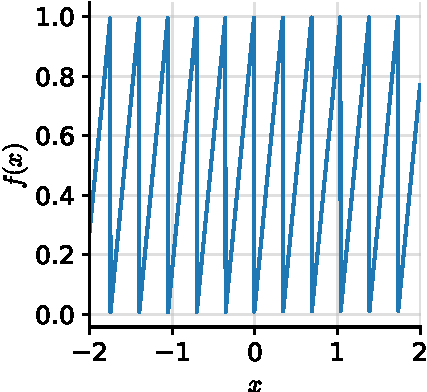
\includegraphics[height=4cm]{\gp{experiments/synthetic_data/sawtooth_x1y1.pdf}}\hfill~
        \caption{$d_x = 1$, $d_y = 1$}
    \end{subfigure}
    \hfill
    \begin{subfigure}{0.63\linewidth}
        \hspace{5pt}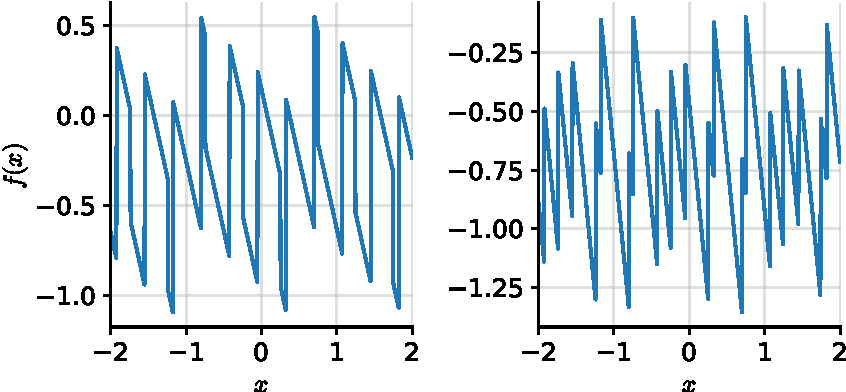
\includegraphics[height=4cm]{\gp{experiments/synthetic_data/sawtooth_x1y2.pdf}}\hfill~
        \caption{$d_x = 1$, $d_y = 2$}
    \end{subfigure}\\[1em]
    \begin{subfigure}{0.36\linewidth}
        ~\hfill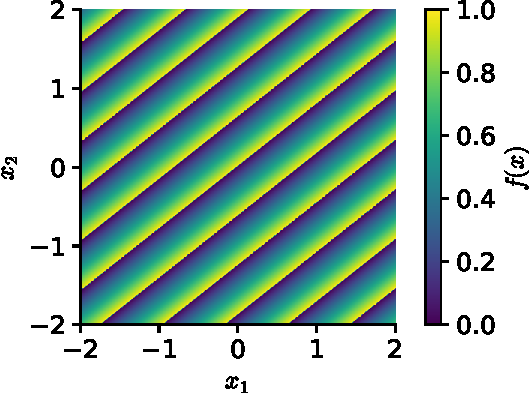
\includegraphics[height=4cm]{\gp{experiments/synthetic_data/sawtooth_x2y1.pdf}}
        \caption{$d_x = 2$, $d_y = 1$}
    \end{subfigure}
    \hfill
    \begin{subfigure}{0.63\linewidth}
        ~\hfill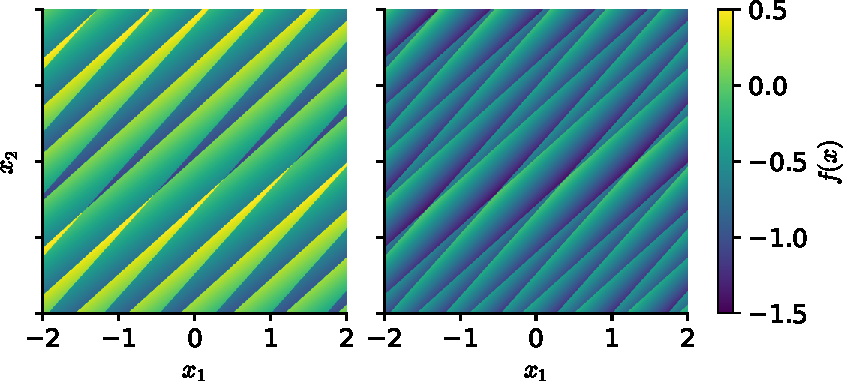
\includegraphics[height=4cm]{\gp{experiments/synthetic_data/sawtooth_x2y2.pdf}}
        \caption{$d_x = 2$, $d_y = 2$}
    \end{subfigure}
    \hfill
    \caption[
        Samples from the sawtooth data process
    ]{
        Samples from the sawtooth data process with one and two-dimensional inputs ($d_x = 1$ and $d_x = 2$) and one and two-dimensional outputs ($d_y = 1$ and $d_y = 2$)
    }
    \label{fig:synthetic_sawtooth}
\end{figure}

We synthetically generate data sets by randomly sampling from five different choices for the ground-truth stochastic process $f$.
Let the inputs be $d_x$-dimensional.
Then define the following stochastic processes:
\begin{itemize}[leftmargin=8em]
    \item[EQ:]
        a Gaussian process with an exponentiated quadratic (EQ) kernel:
        \begin{equation}
           f \sim \GP(0, \exp(-\tfrac1{2\ell^2}\norm{\vx - \vx'}_2^2)) 
        \end{equation}
        where $\ell > 0$ is a length scale;
    \item[Mat\'ern--$\tfrac52$:]
        a Gaussian process with a Mat\'ern--$\tfrac52$ kernel:
        \begin{equation}
           f \sim \GP(0, k(\tfrac1\ell\norm{\vx - \vx'}_2))
        \end{equation}
        where $k(r) = (1 + \sqrt{5}r + \tfrac53 r^2)e^{-r}$
        and $\ell > 0$ is a length scale;
    \item[weakly periodic:]
        a Gaussian process with a weakly periodic kernel:
        \begin{equation}
            f \sim \GP(0, \exp(-\tfrac1{2\ell\ss{d}^2}\norm{\vx - \vx'}_2^2 - \tfrac{2}{\ell\ss{p}^2}\norm{\sin(\tfrac{\pi}{p} (\vx - \vx'))}_2^2))  
        \end{equation}
        where $\ell\ss{d} > 0$ is a length scale specifying how quickly the periodic pattern changes, $\ell\ss{p} > 0$ a length scale of the periodic pattern, and $p > 0$ the period;
        and where the application of $\sin$ is elementwise;
    \item[sawtooth:]
        a sawtooth process with a random frequency, direction, and phase:
        \begin{equation}
             f = \omega \lra{\vx, \vu}_2 + \phi \mod 1
        \end{equation}
        where $\omega \sim \Unif(\Omega)$ is the frequency of the sawtooth wave, $\vu \sim \Unif(\set{\vx \in \R^{d_x} : \norm{\vx}_2 = 1})$ the direction, and $\phi \sim \Unif([0, 1])$ the phase;
    \item[mixture:]
        with equal probability, sample $f$ from the EQ process, Mat\'ern--$\tfrac52$ process, weakly periodic process, or sawtooth process.
\end{itemize}
We will call these stochastic processes the \emph{data processes}.
The data processes are stochastic processes with $d_x$-dimensional inputs and one-dimensional outputs.
We will turn them into processes with $d_y$-dimensional outputs according to the following procedure:
sample from the one-dimensional-output prior $d_y$ times;
and, for these $d_y$ samples, take $d_y$ different linear combinations.
The coefficients of these linear combinations are once independently drawn from $\Normal(0,1)$ and then fixed.
We will consider one ($d_x = 1$) and two-dimensional inputs ($d_x = 2$); and one ($d_y = 1$) and two-dimensional outputs ($d_y = 2$);
yielding four configurations per data process.
Whereas thus far we only considered one-dimensional inputs and outputs,
these configurations will generate context and target sets with potentially multidimensional inputs and outputs.
We choose the parameters of the data processes based on the input dimensionality $d_x$:
\begin{align}
    \ell &= c \cdot\tfrac14, &
    \ell\ss{d} &= c \cdot\tfrac12, &
    \ell\ss{s} &= c, &
    p &= c \cdot\tfrac14, &
    \Omega &= [c^{-1} \cdot 2, c^{-1} \cdot 4]
\end{align}
with $c = \sqrt{d_x}$.
Scaling with the input dimensionality aims to roughly ensure that data with one-dimensional inputs and data with two-dimensional inputs are equally difficult.
\Cref{fig:synthetic_sawtooth} illustrates the sawtooth data process in all four configurations.

We will construct data sets by sampling inputs uniformly at random from
$\X = [-2, 2]^{d_x}$
and then sampling outputs from one of the data processes.
We will colloquially call $\X$ the \emph{training range}.
For the EQ, Mat\'ern--$\frac52$, and weakly periodic process, but not for the sawtooth process\footnote{
    The sawtooth process is already challenging enough.
},
we also add independent Gaussian noise with variance $0.05$.
The numbers of context and target points are as follows.
For the EQ, Mat\'ern--$\frac52$, and weakly periodic process,
the number of context points is chosen uniformly at random from $\set{0, \ldots, 30 \cdot d_x}$ and
the number of targets points is fixed to $50 \cdot d_x$.
For the sawtooth and mixture process,
the number of context points is chosen uniformly at random from $\set{0, \ldots, 75 \cdot d_x}$ and
the number of targets points is fixed to $100 \cdot d_x$.
In the case of a multidimensional-output data process, we separately sample the number and positions of the context and target inputs for every output dimension.

For every data process and each of the four configurations, we train every model from \cref{tab:overview_models} and evaluate the model in three different ways.
First, we evaluate the model on data generated exactly like the training data.
This task is called \emph{interpolation} and abbreviated ``int.'' in the tables of results.
The interpolation task measures how well a model fits the data
and is the primary measure of performance.
Second, we evaluate the model on data with inputs sampled from $[2, 6]^{d_x}$.
This task is called \emph{out-of-input-distribution (OOID) interpolation} and abbreviated ``OOID'' in the tables of results.
OOID interpolation measures how well a model generalises to data sampled from other regions of the input space.
Third, we evaluate the model on data with context inputs sampled from $[-2, 2]^{d_x}$ and target inputs sampled from $[2, 6]^{d_x}$.
This task is called \emph{extrapolation} and abbreviated ``ext.'' in the tables of results.
The extrapolation task measures how well predictions based on data in the training range generalise to other regions of the input space.

Further details on the setup and execution of this experiment can be found in
\cref{\xrprefix{sec:experimental_details:models},\xrprefix{sec:experimental_details:protocols},\xrprefix{sec:experimental_details:synthetic}}.
\Cref{\xrprefix{sec:experimental_details:models}} describes the general architectures of the models, \cref{\xrprefix{sec:experimental_details:protocols}} describes the general training, cross-validation, and evaluation protocols, and \cref{\xrprefix{sec:experimental_details:synthetic}} describes details specific to this experiment.

\paragraph{Results}
In the description of the results, we call the experiments with the EQ, Mat\'ern--$\frac52$, and weakly periodic processes the \emph{Gaussian experiments} and the experiments with the sawtooth and mixture processes the \emph{non-Gaussian experiments}.
On the page after next page,
\Cref{tab:synthetic_Gaussian} summarises the results of the Gaussian experiments, and \cref{tab:synthetic_non-Gaussian} summarises the results of the non-Gaussian experiments.
After these summaries, the next ten pages show the full results:
\Cref{tab:synthetic_eq-1,tab:synthetic_eq-2} tabulate the results for the EQ process,
\cref{tab:synthetic_matern-1,tab:synthetic_matern-2} tabulate the results for the Mat\'ern--$\frac52$ process,
\cref{tab:synthetic_weakly-periodic-1,tab:synthetic_weakly-periodic-2} tabulate the results for the weakly periodic process,
\cref{tab:synthetic_sawtooth-1,tab:synthetic_sawtooth-2} tabulate the results for the sawtooth process, and
\cref{tab:synthetic_mixture-1,tab:synthetic_mixture-2} tabulate the results for the mixture process.

\paragraph{A word of caution}
After this page, we will proceed to present all aforementioned tables.
The description of the results started in the next paragraph will continue after these tables.
In the tables, every LNP occurs three times, corresponding to different combinations of training and evaluation objectives;
see \cref{\xrprefix{sec:experimental_details:protocols}}.
As this thesis is primarily concerned with non-latent-variable neural processes, we will consider the performance of an LNP to simply be the best of the three numbers.

\newcommand{\onedtwoddescription}{
    Shows for one-dimensional inputs (1D; $d_x=1$) and two-dimensional inputs (2D; $d_y=2$) the performance for
    interpolation within the range $[-2, 2]^{d_x}$ where the models were trained  (``Int.'');
    interpolation within the range $[2, 6]^{d_x}$ which the models have never seen before (``OOID'');
    and extrapolation from the range $[-2, 2]^{d_x}$ to the range $[2, 6]^{d_x}$ (``Ext.'').
    Models are ordered by interpolation performance for one-dimensional inputs.
}
\newcommand{\oneddescription}{
    Shows for one-dimensional outputs ($d_y=1$) and two-dimensional outputs ($d_y=2$) the performance for
    interpolation within the range $[-2, 2]$ where the models where trained  (``Int.'');
    interpolation within the range $[2, 6]$ which the models have never seen before (``OOID'');
    and extrapolation from the range $[-2, 2]$ to the range $[2, 6]$ (``Ext.'').
    Models are ordered by interpolation performance.
}
\newcommand{\twoddescription}{
    Shows for one-dimensional outputs ($d_y=1$) and two-dimensional outputs ($d_y=2$) the performance for
    interpolation within the range $[-2, 2]^2$ where the models where trained  (``Int.'');
    interpolation within the range $[2, 6]^2$ which the models have never seen before (``OOID'');
    and extrapolation from the range $[-2, 2]^2$ to the range $[2, 6]^2$ (``Ext.'').
    Models are ordered by interpolation performance.
}
\newcommand{\latentvariabledescription}{
    The latent variable models are trained and evaluated with the ELBO objective (ELBO);
    trained and evaluated with the ML objective (ML);
    and trained with the ELBO objective and evaluated with the ML objective (ELBO--ML; E.--M.).
}
\newcommand{\convabbrevdescription}{
    ``Conv'' is abbreviated with ``Cv''.
}
\newcommand{\numbersdescription}{
    Errors indicate the central 95\%-confidence interval.
    Numbers which are significantly best ($p < 0.05$) are boldfaced.
    Numbers which are very large are marked as failed with ``F''.
    Numbers which are missing could not be run.
}
\newcommand{\diagonaldescription}{
    Diagonal GP refers to predictions by the ground-truth Gaussian processes without correlations.
}
\newcommand{\trivialdescription}{
    Trivial refers to predicting the empirical means and standard deviation of the test data.
}

\begin{table}[t]
    \centering
    \caption
    [
        Summary of results for the Gaussian synthetic experiments
    ]
    {
        For the Gaussian experiments, average Kullback--Leibler divergences of the posterior prediction map $\pi_f$ with respect to the model normalised by the number of target points.
        \onedtwoddescription
        \latentvariabledescription
        \diagonaldescription
        \trivialdescription
        \numbersdescription
    }
    \label{tab:synthetic_Gaussian}
    \small
    \setlength{\tabcolsep}{3pt}
    \subimport{tables/}{synthetic_gaussian_average.tex}
\end{table}

\begin{table}[t]
    \centering
    \caption
    [
        Summary of results for the non-Gaussian synthetic experiments
    ]
    {
        For the non-Gaussian experiments, average log-likelihoods normalised by the number of target points.
        \onedtwoddescription
        \latentvariabledescription
        \trivialdescription
        \numbersdescription
    }
    \label{tab:synthetic_non-Gaussian}
    \small
    \setlength{\tabcolsep}{3pt}
    \subimport{tables/}{synthetic_non-gaussian_average.tex}
\end{table}

\begin{table}[t]
    \centering
    \caption
    [
        Results for the EQ synthetic experiments with 1D inputs
    ]
    {
        For the EQ synthetic experiments with one-dimensional inputs, average Kullback--Leibler divergences of the posterior prediction map $\pi_f$ with respect to the model normalised by the number of target points.
        \oneddescription
        \latentvariabledescription
        \diagonaldescription
        \trivialdescription
        \numbersdescription
    }
    \label{tab:synthetic_eq-1}
    \footnotesize
    \setlength{\tabcolsep}{2pt}
    \subimport{tables/}{synthetic_eq1-1.tex}
    \subimport{tables/}{synthetic_eq1-2.tex}
\end{table}

\begin{table}[t]
    \centering
    \caption
    [
        Results for the EQ synthetic experiments with 2D inputs
    ]
    {
        For the EQ synthetic experiments with two-dimensional inputs, average Kullback--Leibler divergences of the posterior prediction map $\pi_f$ with respect to the model normalised by the number of target points.
        \twoddescription
        \latentvariabledescription
        \diagonaldescription
        \trivialdescription
        \numbersdescription
    }
    \label{tab:synthetic_eq-2}
    \footnotesize
    \setlength{\tabcolsep}{2pt}
    \subimport{tables/}{synthetic_eq2-1.tex}
    \subimport{tables/}{synthetic_eq2-2.tex}
\end{table}

\begin{table}[t]
    \centering
    \caption
    [
        Results for the Mat\'ern--$\tfrac52$ synthetic experiments with 1D inputs
    ]
    {
        For the Mat\'ern--$\frac52$ synthetic experiments with one-dimensional inputs, average Kullback--Leibler divergences of the posterior prediction map $\pi_f$ with respect to the model normalised by the number of target points.
        \oneddescription
        \latentvariabledescription
        \diagonaldescription
        \trivialdescription
        \numbersdescription
    }
    \label{tab:synthetic_matern-1}
    \footnotesize
    \setlength{\tabcolsep}{2pt}
    \subimport{tables/}{synthetic_matern1-1.tex}
    \subimport{tables/}{synthetic_matern1-2.tex}
\end{table}

\begin{table}[t]
    \centering
    \caption
    [
        Results for the Mat\'ern--$\tfrac52$ synthetic experiments with 2D inputs
    ]
    {
        For the Mat\'ern--$\frac52$ synthetic experiments with two-dimensional inputs, average Kullback--Leibler divergences of the posterior prediction map $\pi_f$ with respect to the model normalised by the number of target points.
        \twoddescription
        \diagonaldescription
        \trivialdescription
        \numbersdescription
    }
    \label{tab:synthetic_matern-2}
    \footnotesize
    \setlength{\tabcolsep}{2pt}
    \subimport{tables/}{synthetic_matern2-1.tex}
    \subimport{tables/}{synthetic_matern2-2.tex}
\end{table}

\begin{table}[t]
    \centering
    \caption
    [
        Results for the weakly periodic synthetic experiments with 1D inputs
    ]
    {
        For the weakly periodic synthetic experiments with one-dimensional inputs, average Kullback--Leibler divergences of the posterior prediction map $\pi_f$ with respect to the model normalised by the number of target points.
        \oneddescription
        \latentvariabledescription
        \diagonaldescription
        \trivialdescription
        \numbersdescription
    }
    \label{tab:synthetic_weakly-periodic-1}
    \footnotesize
    \setlength{\tabcolsep}{2pt}
    \subimport{tables/}{synthetic_weakly-periodic1-1.tex}
    \subimport{tables/}{synthetic_weakly-periodic1-2.tex}
\end{table}

\begin{table}[t]
    \centering
    \caption
    [
        Results for the weakly periodic synthetic experiments with 2D inputs
    ]
    {
        For the weakly periodic synthetic experiments with two-dimensional inputs, average Kullback--Leibler divergences of the posterior prediction map $\pi_f$ with respect to the model normalised by the number of target points.
        \twoddescription
        \latentvariabledescription
        \diagonaldescription
        \trivialdescription
        \numbersdescription
    }
    \label{tab:synthetic_weakly-periodic-2}
    \footnotesize
    \setlength{\tabcolsep}{2pt}
    \subimport{tables/}{synthetic_weakly-periodic2-1.tex}
    \subimport{tables/}{synthetic_weakly-periodic2-2.tex}
\end{table}

\begin{table}[t]
    \centering
    \caption
    [
        Results for the sawtooth synthetic experiments with 1D inputs
    ]
    {
        For the sawtooth synthetic experiments with one-dimensional inputs, average log-likelihoods normalised by the number of target points.
        \oneddescription
        \latentvariabledescription
        \convabbrevdescription
        \trivialdescription
        \numbersdescription
    }
    \label{tab:synthetic_sawtooth-1}
    \footnotesize
    \setlength{\tabcolsep}{2pt}
    \subimport{tables/}{synthetic_sawtooth1-1.tex}%
    \subimport{tables/}{synthetic_sawtooth1-2.tex}
\end{table}

\begin{table}[t]
    \centering
    \caption
    [
        Results for the sawtooth synthetic experiments with 2D inputs
    ]
    {
        For the sawtooth synthetic experiments with two-dimensional inputs, average log-likelihoods normalised by the number of target points.
        \twoddescription
        \latentvariabledescription
        \convabbrevdescription
        \trivialdescription
        \numbersdescription
    }
    \label{tab:synthetic_sawtooth-2}
    \footnotesize
    \setlength{\tabcolsep}{2pt}
    \subimport{tables/}{synthetic_sawtooth2-1.tex}%
    \subimport{tables/}{synthetic_sawtooth2-2.tex}
\end{table}

\begin{table}[t]
    \centering
    \caption
    [
        Results for the mixture synthetic experiments with 1D inputs
    ]
    {
        For the mixture synthetic experiments with one-dimensional inputs, average log-likelihoods normalised by the number of target points.
        \oneddescription
        \latentvariabledescription
        \convabbrevdescription
        \trivialdescription
        \numbersdescription
    }
    \label{tab:synthetic_mixture-1}
    \footnotesize
    \setlength{\tabcolsep}{2pt}
    \subimport{tables/}{synthetic_mixture1-1.tex}%
    \subimport{tables/}{synthetic_mixture1-2.tex}
\end{table}

\begin{table}[t]
    \centering
    \caption
    [
        Results for the mixture synthetic experiments with 2D inputs
    ]
    {
        For the mixture synthetic experiments with two-dimensional inputs, average log-likelihoods normalised by the number of target points.
        \twoddescription
        \latentvariabledescription
        \convabbrevdescription
        \trivialdescription
        \numbersdescription
    }
    \label{tab:synthetic_mixture-2}
    \footnotesize
    \setlength{\tabcolsep}{2pt}
    \subimport{tables/}{synthetic_mixture2-1.tex}%
    \subimport{tables/}{synthetic_mixture2-2.tex}
\end{table}

\afterpage{\FloatBarrier}

\paragraph{Performance of CNPs in Gaussian experiments}
\looseness=-1
In the Gaussian experiments, the ground-truth $f$ is a Gaussian process, so we can compute the conditional neural process approximation (CNPA; \cref{\xrprefix{def:cnpa}}).
Recall that the CNPA is what a CNP converges to in the limit of infinite data;
the CNPA provides an upper bound on the performance of a CNP.
The CNPA is given by taking the mean map (\cref{\xrprefix{def:mean_map}}) and variance map (\cref{\xrprefix{def:variance_map}}) of the posterior prediction map (\cref{\xrprefix{prop:cnpa_characterisation}}). \index{neural process approximation!conditional}
Taking the variance map rather than the kernel map (\cref{\xrprefix{def:kernel_map}}) discards correlations,
so the CNPA is, in some sense, a \emph{diagonalised} version of the posterior prediction map $\pi_f$.
This diagonalised version of $\pi_f$, which is equal to the CNPA, is listed as ``\emph{Diagonal GP}'' in \cref{tab:synthetic_Gaussian,tab:synthetic_eq-1,tab:synthetic_eq-2,tab:synthetic_matern-1,tab:synthetic_matern-2,tab:synthetic_weakly-periodic-1,tab:synthetic_weakly-periodic-2}.

\Cref{tab:synthetic_Gaussian} summarises the results of the Gaussian experiments.
For the task of interpolation, the ConvCNP is, for all six summary statistics, 0.00--0.01 away from the CNPA.
This means that the ConvCNP is able to consistently recover the CNPA.
In contrast, the ACNP comes close, but is not quite able to converge onto the CNPA;
and the CNP is not able to come close at all.
%
For OOID interpolation, the performance of the ACNP and CNP deteriorates.
The ConvCNP, on the other hand, performs equally well in the interpolation and OOID interpolation tasks.
This clearly demonstrates the benefits of translation equivariance,
which allows ConvCNP to generalise to unseen parts of the input space. 

Amongst the Gaussian experiments, the weakly periodic process appears to be the more challenging one.
For the EQ and weakly periodic process, \cref{fig:synthetic_cnps} compares predictions from the CNP, ACNP, and ConvCNP, showing that only the ConvCNP consistently recovers the CNPA and only the ConvCNP successfully generalises beyond the training range. 

\paragraph{Performance of GNPs in Gaussian experiments}
Since the ground-truth stochas\-tic process $f$ is Gaussian, the Gaussian neural process approximation (GNPA; \cref{\xrprefix{def:gnpa}}) is equal to the posterior prediction map $\pi_f$. \index{neural process approximation!Gaussian}
Therefore, in the limit of infinite data, GNPs should have the capacity the recover the posterior prediction map, the best possible outcome.
\Cref{tab:synthetic_Gaussian} shows that the FullConvGNP consistently recovers the posterior prediction map $\pi_f$ for one-dimensional inputs.
For two-dimensional inputs, the FullConvGNP is computationally too expensive, unfortunately, so it cannot be run (\cref{\xrprefix{sec:convcnps:conclusion}}).
In terms of interpolation performance, the ConvGNP performs second best, followed by the AGNP, and the GNP comes last.
Note, however, that no GNP is able to consistently recover the posterior prediction map in all cases.

In \cref{tab:synthetic_Gaussian}, all GNPs perform better than the CNPA, which means that all GNPs successfully exploit correlations to achieve performances unachievable by models that do not model correlations.
In comparison, the LNPs struggle to outperform the CNPA.
Comparing GNPs and LNPs in the more detailed results, \cref{tab:synthetic_eq-1,tab:synthetic_eq-2,tab:synthetic_matern-1,tab:synthetic_matern-2,tab:synthetic_weakly-periodic-1,tab:synthetic_weakly-periodic-2} show that GNPs consistently perform better than their latent-variable counterparts,
demonstrating the benefits of GNPs when the ground truth really is Gaussian.
In the most difficult Gaussian experiment, the weakly periodic process with two-dimensional inputs and outputs,
\cref{tab:synthetic_weakly-periodic-2} shows that the ConvGNP is the only GNP to consistently outperform the CNPA;
and no other GNP and no LNP is able to outperform the CNPA.
In this most difficult case, however, even though ConvGNP performs best amongst all GNPs and LNPs, the ConvGNP is not able to come close to the posterior prediction map.

In terms of generalisation performance,
\cref{tab:synthetic_Gaussian} shows that
the ConvGNP and FullConvGNP perform equally well in the interpolation and OOID interpolation tasks,
whereas the performance of the GNP and AGNP deteriorate for OOID interpolation.
This behaviour is expected:
the ConvGNP and FullConvGNP have a built-in mechanism to generalise to unseen parts of the input space,
but the GNP and AGNP do not.

\begin{figure}[t]
    \centering
    \begin{subfigure}{\linewidth}
        \centering
        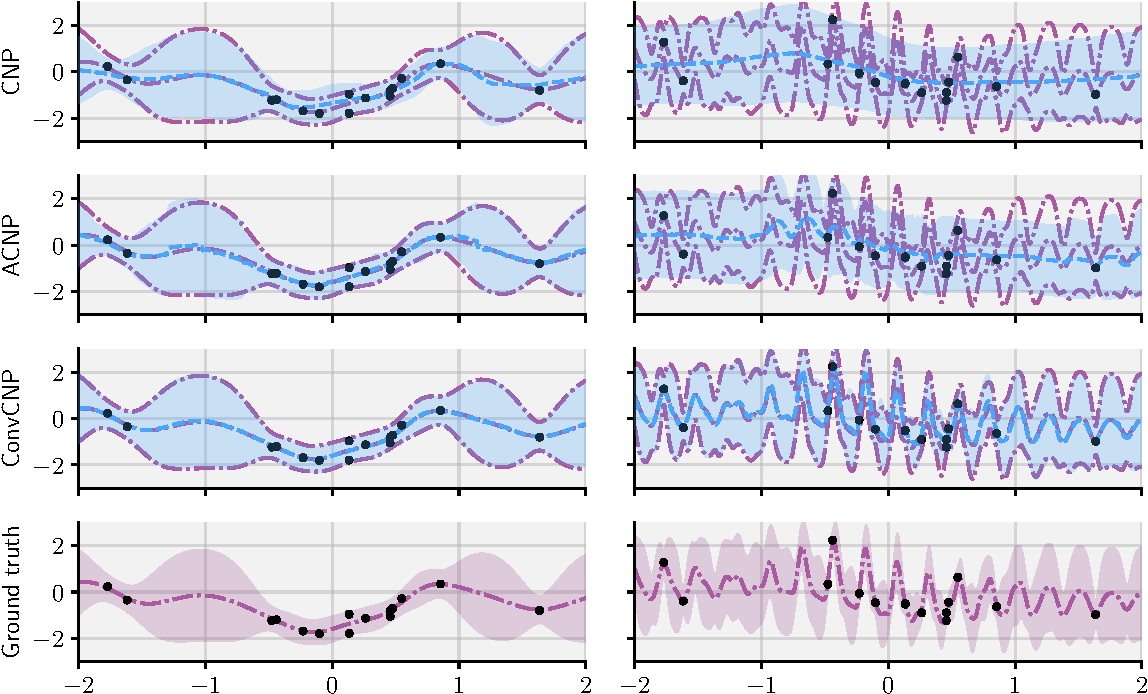
\includegraphics[width=\linewidth]{\gp{experiments/synthetic_cnp/cnps_inside.pdf}}
        \caption{Predictions and observations inside the training range}
    \end{subfigure} \\[1em]
    \begin{subfigure}{\linewidth}
        \centering
        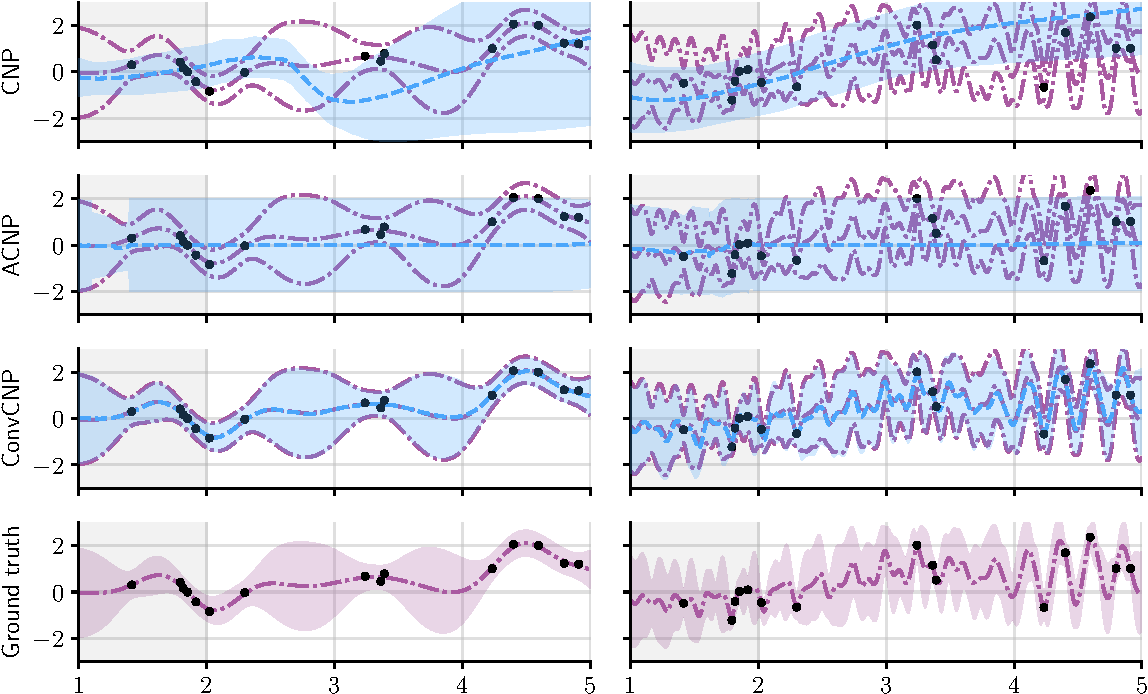
\includegraphics[width=\linewidth]{\gp{experiments/synthetic_cnp/cnps_outside.pdf}}
        \caption{Predictions and observations partly inside and partly outside the training range}
    \end{subfigure}
    \caption[
        Predictions by CNPs in the Gaussian synthetic experiments
    ]{
        Predictions by CNPs in the Gaussian synthetic experiments.
        \emph{Left column:} data sampled from the EQ data process.
        \emph{Right column:} data sampled from the weakly-periodic data process.
        The training range is shaded grey.
        Shows predictions by the models in dashed blue and predictions by the ground truth in dot-dashed purple.  % Standard
        Filled regions are central 95\%-credible regions.

    }
    \label{fig:synthetic_cnps}
\end{figure}

\begin{figure}[t]
    \centering
    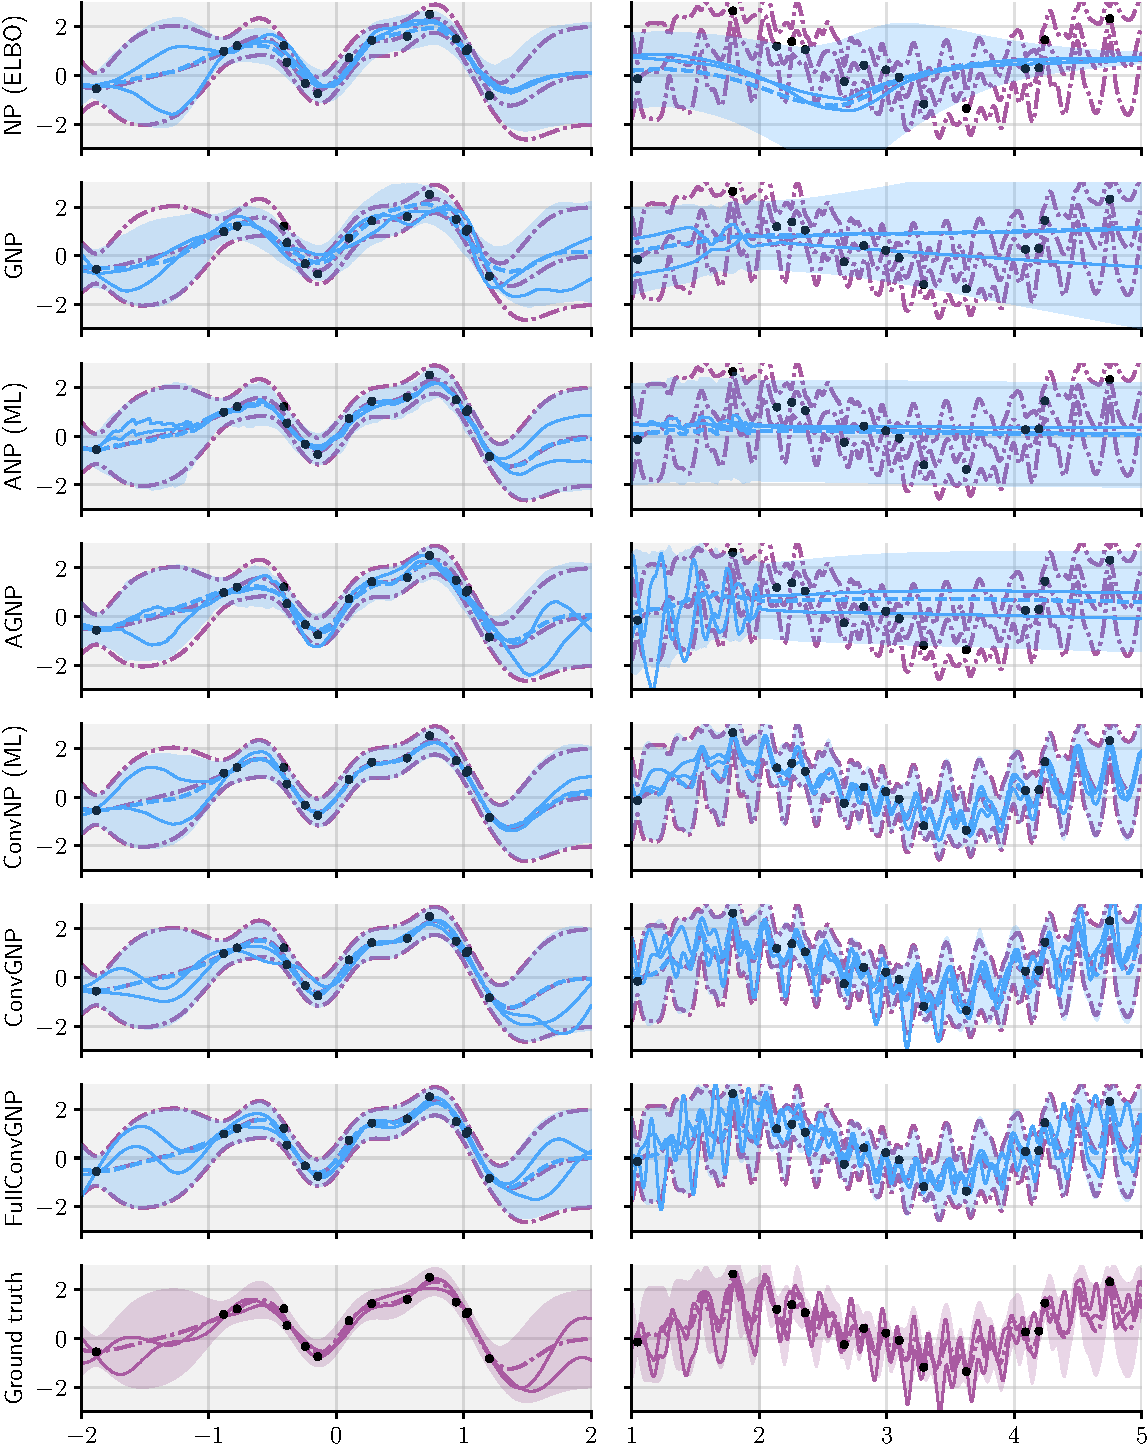
\includegraphics[width=\linewidth]{\gp{experiments/synthetic_gnp/gnps.pdf}}
    \caption[
        Predictions by LNPs and GNPs in the Gaussian synthetic experiments
    ]{
        Predictions by LNPs and GNPs in the Gaussian synthetic experiments.
        \emph{Left column:} data sampled from the EQ data process.
        \emph{Right column:} data sampled from the weakly-periodic data process.
        The training range is shaded grey.
        Shows predictions by the models in dashed blue and predictions by the ground truth in dot-dashed purple.  % Standard
        Filled regions are central 95\%-credible regions.

    }
    \label{fig:synthetic_gnps}
\end{figure}
\begin{figure}[t]
    \centering
    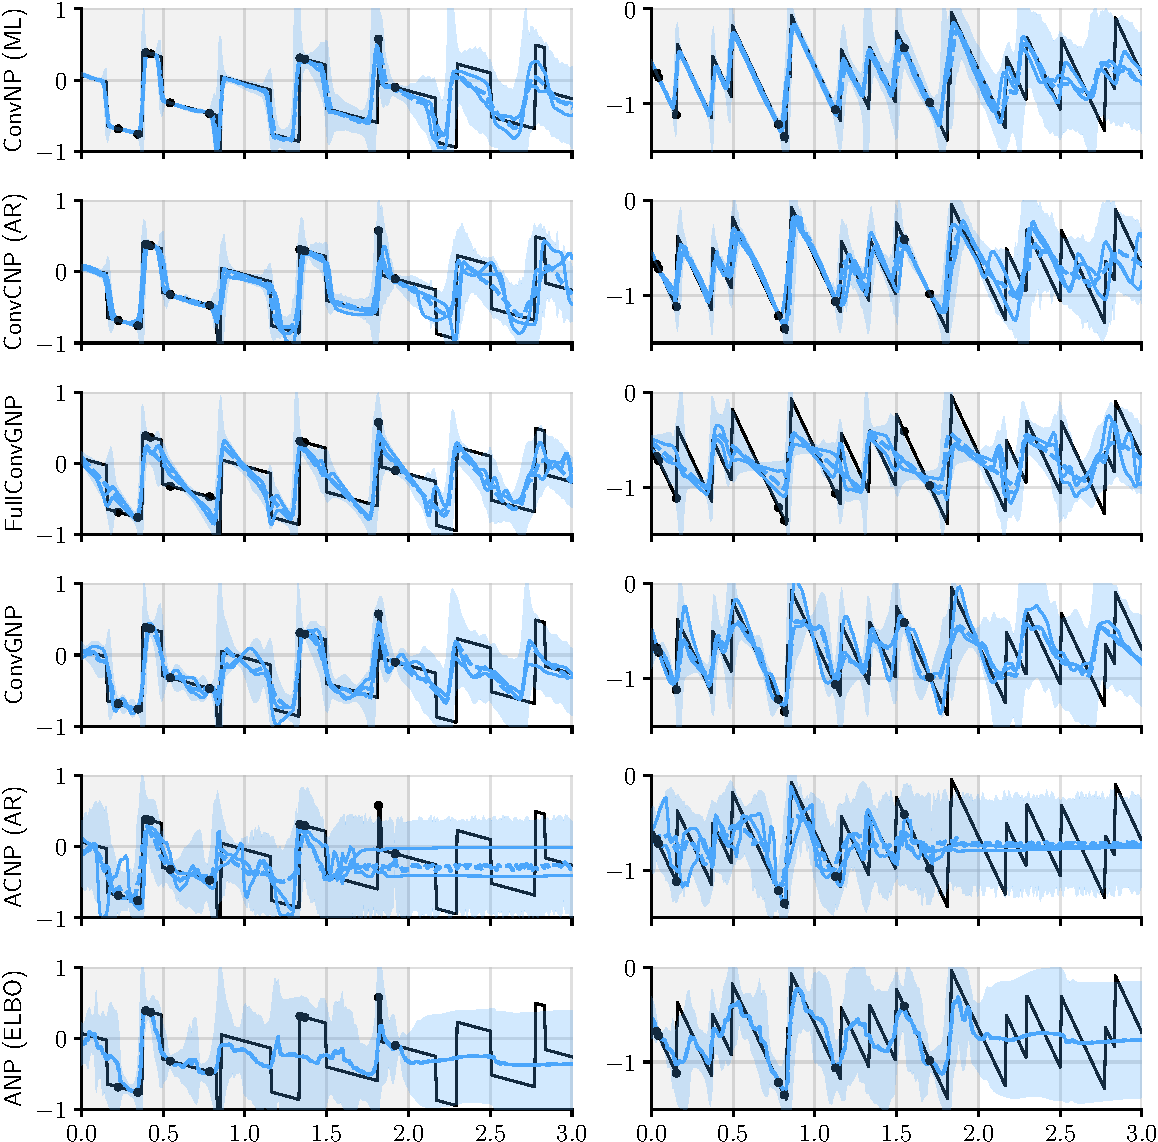
\includegraphics[width=\linewidth]{\gp{experiments/synthetic_sawtooth/sawtooth.pdf}}
    \caption[
        Predictions by the best-performing models in the sawtooth synthetic exp.\
    ]{
        Predictions by the best-performing models in the sawtooth synthetic experiment with one-dimensional inputs and two-dimensional outputs (\cref{tab:synthetic_sawtooth-1}).
        For both outputs, the models observe 20 data points randomly sampled from $[-2, 2]$;
        the plots only show the observations on $[0, 2]$.
        \emph{Left column:} first output of the sawtooth process.
        \emph{Right column:} second output of the sawtooth process.
        The training range is shaded grey.
        Filled regions are central 95\%-credible regions.
    }

    \label{fig:synthetic_non-Gaussian_sawtooth}
\end{figure}
\begin{figure}[t]
    \centering
    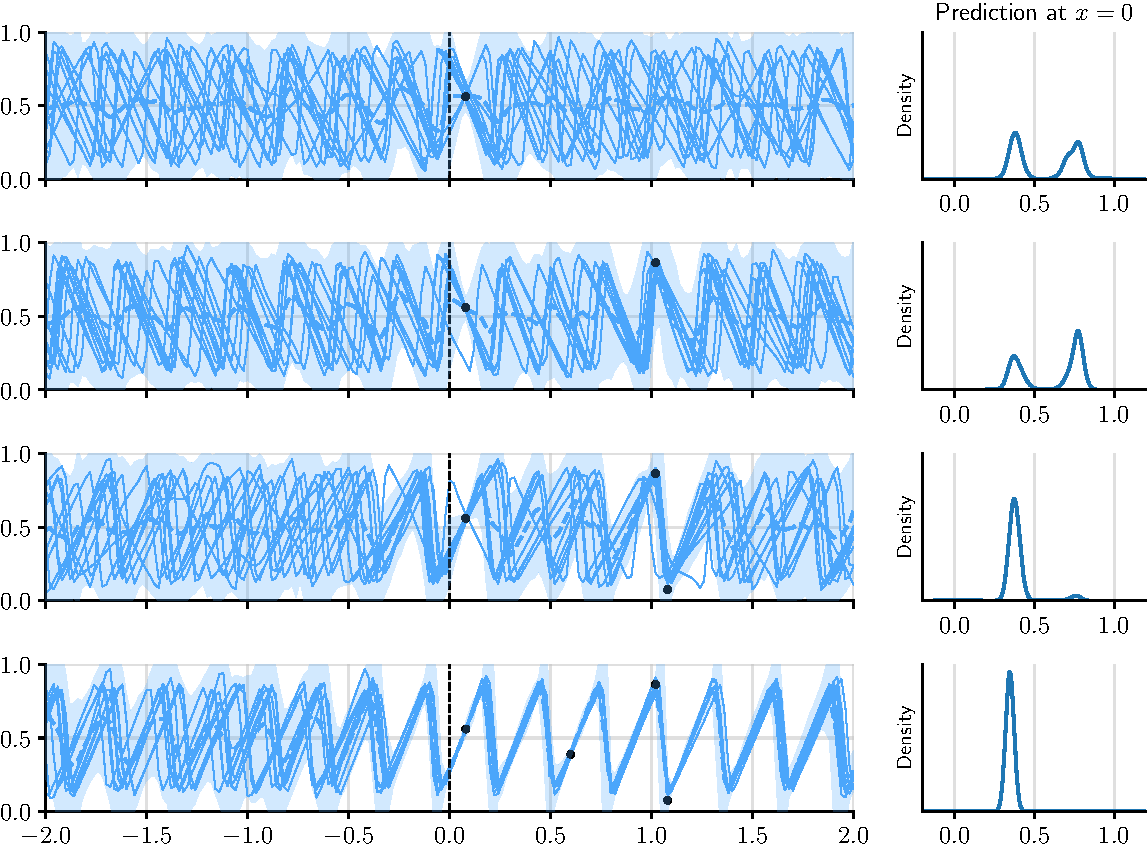
\includegraphics[width=\linewidth]{\gp{experiments/synthetic_sawtooth_collapse/sawtooth_collapse.pdf}}
    \caption[
        Multi-modality of predictions by the AR ConvCNP
    ]{
        Multi-modality of predictions by the AR ConvCNP.
        Shows four observations sampled from the sawtooth process.
        In the four rows, these four observations are revealed one data point at a time.
        Every row also shows a kernel density estimate of the prediction at $x = 0$.
        Note that the prediction is bimodal for one and two observations, and collapses to a single mode upon observing the third observation.
        Filled regions are central 95\%-credible regions.

    }
    \label{fig:synthetic_non-Gaussian_sawtooth_collape}
\end{figure}

\afterpage{\FloatBarrier}

However, in terms of generalisation performance, there is one important anomaly:
the ConvGNP performs well on OOID interpolation,
but the model's performance for extrapolation is consistently poor.
This shows in \cref{tab:synthetic_Gaussian} as well as in the more detailed results, \cref{tab:synthetic_eq-1,tab:synthetic_eq-2,tab:synthetic_matern-1,tab:synthetic_matern-2,tab:synthetic_weakly-periodic-1,tab:synthetic_weakly-periodic-2}.
What is going wrong is that the ConvGNP implements the eigenmap (\cref{\xrprefix{def:eigenmap}}) with the convolutional deep set from \cref{\xrprefix{thm:conv_deep_set}}, and the output of this convolutional deep set becomes constant when it is far away from the context inputs.
This problem is exactly what the FullConvGNP's additional source channel solves, so this problem is not present for the FullConvGNP.
We might hope to fix this flaw of the ConvGNP by also incorporating a source channel,
but it is not clear what a source channel would look like for the ConvGNP.
On a deeper level, this flaw of the ConvGNP is a consequence of that a DTE kernel map might not have a TE eigenmap.
See \cref{\xrprefix{sec:convcnps:gnp}} for a more detailed discussion of problems with the representational capacity of the ConvGNP. \index{representational capacity}
We again emphasise that these issues---theoretical in \cref{\xrprefix{sec:convcnps:gnp}}, but now practical here---underline the importance of entirely basing neural process architectures on representation theorems.

For the EQ data process and weakly-periodic data process,
\Cref{fig:synthetic_gnps} compares predictions of LNPs and GNPs.

\paragraph{Performance of AR CNPs in Gaussian experiments}
Having analysed the performance of CNPs and GNPs, we add AR CNPs to the mix.
In terms of interpolation performance, \cref{tab:synthetic_Gaussian} shows that the AR CNP performs better than the CNP; that the AR ACNP performs better than the ACNP; and that the AR ConvCNP performs better than the ConvCNP.
In fact, whereas the ACNP and ConvCNP perform no better and cannot perform better than the CNPA, the AR ACNP and AR ConvCNP significantly outperform the CNPA.
This demonstrates that rolling out a CNP autoregressively can improve performance by successfully modelling dependencies between target outputs.

For Gaussian data,
an important question is which of the classes CNPs, GNPs, LNPs, and AR CNPs should preferably be used.
For the deep-set-based and attentive families, \cref{tab:synthetic_Gaussian} shows that the GNPs perform best overall.
For the convolutional family, however, the AR ConvCNP performs best.
Amongst all neural process models, for one-dimensional inputs, the FullConvGNP performs best, with the AR ConvCNP a close second;
\looseness=-1
and for two-dimensional inputs, the AR ConvCNP performs best.
For two-dimensional inputs, the AR ConvCNP is the only model able to recover the posterior prediction map, an impressive achievement.

In these synthetic experiments, the number of target points is at most 200.
It might be that this number is low enough for the inconsistency of AR CNPs (\cref{\xrprefix{sec:convcnps:ar}}) to not be a problem.
It is possible that, if this number is increased, the performance of AR CNPs deteriorates, whereas the performance of CNPs, GNPs, and LNPs should remain the same.
\looseness=-1
We do not perform evaluation with more than 200 target points, because, at 200 target points, a single evaluation of an AR CNP already takes around two hours in the worst case.

\paragraph{Performance in non-Gaussian experiments}
Whereas the FullConvGNP dominated the leaderboard in the Gaussian experiments, in the non-Gaussian experiments, 
the models' relative performances are different.
\Cref{tab:synthetic_non-Gaussian} summarises the non-Gaussian experiments.
Note that \cref{tab:synthetic_non-Gaussian} shows log-likelihoods rather than Kullback--Leibler divergences:
the posterior prediction map is intractable for non-Gaussian ground-truth stochastic processes.

To begin with, for one-dimensional inputs, the top position is now shared by the AR ConvCNP and ConvNP.
Notably, the AR ConvCNP and ConvNP are both non-Gaussian models.
Previously, in the Gaussian experiments, the best performing GNPs, ConvGNP and FullConvGNP, outperformed all LNPs.
Now, in the non-Gaussian experiments, the best performing LNP, the ConvNP, outperforms all GNPs.
This shows that the Gaussianity assumption of GNPs helps when the ground truth really is Gaussian,
but hurts when the data is non-Gaussian.
For two-dimensional inputs, the AR ConvCNP strongly outperforms all other models.

For the sawtooth data with one-dimensional inputs and outputs, \cref{tab:synthetic_sawtooth-1} shows that the non-convolutional CNPs and GNPs completely failed to capture any structure of the data.
Only the non-convolutional neural processes using a latent variable were able to achieve non-trivial performance.
Remarkably, when the output dimension is then increased to two, all models except the CNP achieve non-trivial performance.
This could be due to an increase in number of target points, or perhaps due to increased model capacity;
namely, the architectures of non-convolutional CNPs and GNPs are slightly different for one and two-dimensional outputs (\cref{\xrprefix{sec:experimental_details:models}}).
For the sawtooth data with two-dimensional inputs, \cref{tab:synthetic_sawtooth-2} shows that only the convolutional neural processes achieves non-trivial performance.
All non-convolutional neural processes were unsuccessful in fitting any non-trivial aspect of the data.

\afterpage{\FloatBarrier}

Compared to the Gaussian experiments, the results of the non-Gaussian experiments are generally more variable.
For example, whereas the AR ConvCNP is amongst the best in most non-Gaussian experiments,
\cref{tab:synthetic_mixture-1} shows that it ranks fourth in on the mixture data with one-dimensional inputs and two-dimensional outputs, ranking even behind the ConvGNP.
This variability could be due to imperfect training, due to the fact that we are comparing log-likelihoods rather than Kullback--Leibler divergences, or even due to increased variability between the non-Gaussian data processes.

Finally, we remark that the AR ConvCNP exhibits unparalleled extrapolation performance.
For example, for two-dimensional inputs, \cref{tab:synthetic_non-Gaussian} the AR ConvCNP achieves log-likelihood $0.29$ on average, whereas the second best, the ConvNP, achieves $-0.62$ on average, a difference of $0.91$!
We hypothesise that this exceptional performance is due to the AR ConvCNP's ability to ``renew'' the receptive field, which we explain now.
The non-autoregressive convolutional models are all limited by the receptive field of the CNN architecture (\cref{\xrprefix{def:receptive_field}}):
due to the finite size of the convolutional filters, signals deriving from the context set carry only limitedly far (\cref{\xrprefix{sec:convcnps:generalisation}}).
This limits the model's ability to extrapolate.
\looseness=-1
When the ConvCNP is sampled, however, and this sample is fed back into the architecture (\cref{\xrprefix{proc:ar}}), this produces a new signal starting at the input of that sample.
Hence, at every autoregressive sampling step, the AR ConvCNP effectively ``renews'' the receptive field.

\Cref{fig:synthetic_non-Gaussian_sawtooth}
compares predictions by the best-performing models in the sawtooth synthetic experiment with one-dimensional inputs ($d_x=1$) and two-dimensional outputs ($d_y=2$); see \cref{tab:synthetic_sawtooth-1}.
Moreover, \cref{fig:synthetic_non-Gaussian_sawtooth_collape} illustrates the that, although the predictions of the ConvCNP are Gaussian, the AR ConvCNP can produce appropriate multi-modal predictions.

\section{Sim-to-Real Transfer with the Lotka--Volterra Equations}
\label{sec:experiments:predprey}

\index{sim-to-real transfer}
In this second experiment, we investigate the ability of neural processes to perform sim-to-real transfer.
The goal of sim-to-real transfer is to use a data simulator to make predictions for real data.
There are no requirements on the data simulator:
it can be arbitrarily complicated and involve niche expert knowledge.
Because of the complexity of the data simulator, it usually is not possible to directly use the simulator to make predictions.
The strategy of sim-to-real transfer is to train a model on data generated with the data simulator.
After the model is trained on this synthetic source of data, the model is applied to real data.
In this way, the model facilitates a mechanism in which complex data simulators can be used to make predictions.

\begin{figure}[t]
    \centering
    \small
    \begin{subfigure}{\linewidth}
        \centering
        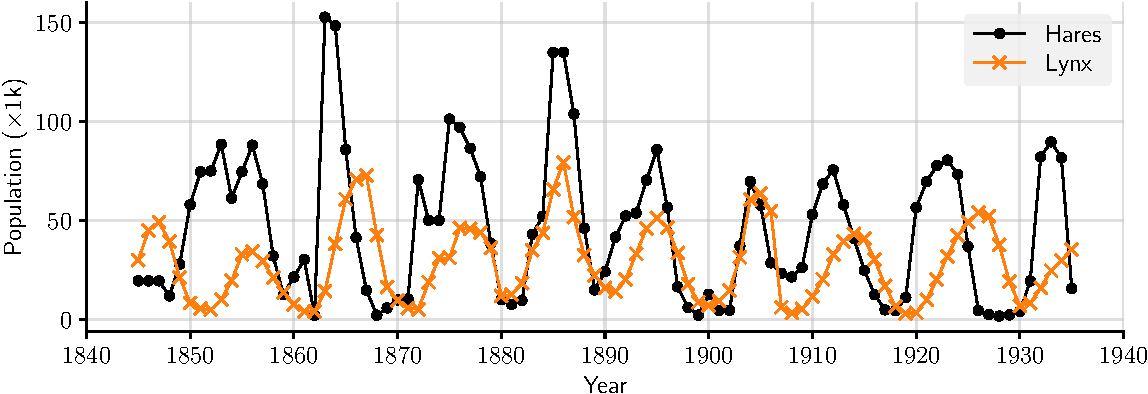
\includegraphics[width=0.8\linewidth]{\gp{experiments/predprey_data/data.pdf}}
        \caption{
            Illustration of the hare--lynx data set
        }
        \label{fig:hare-lyxn_data}
    \end{subfigure} \\[1em]
    \begin{subfigure}{\linewidth}
        \centering
        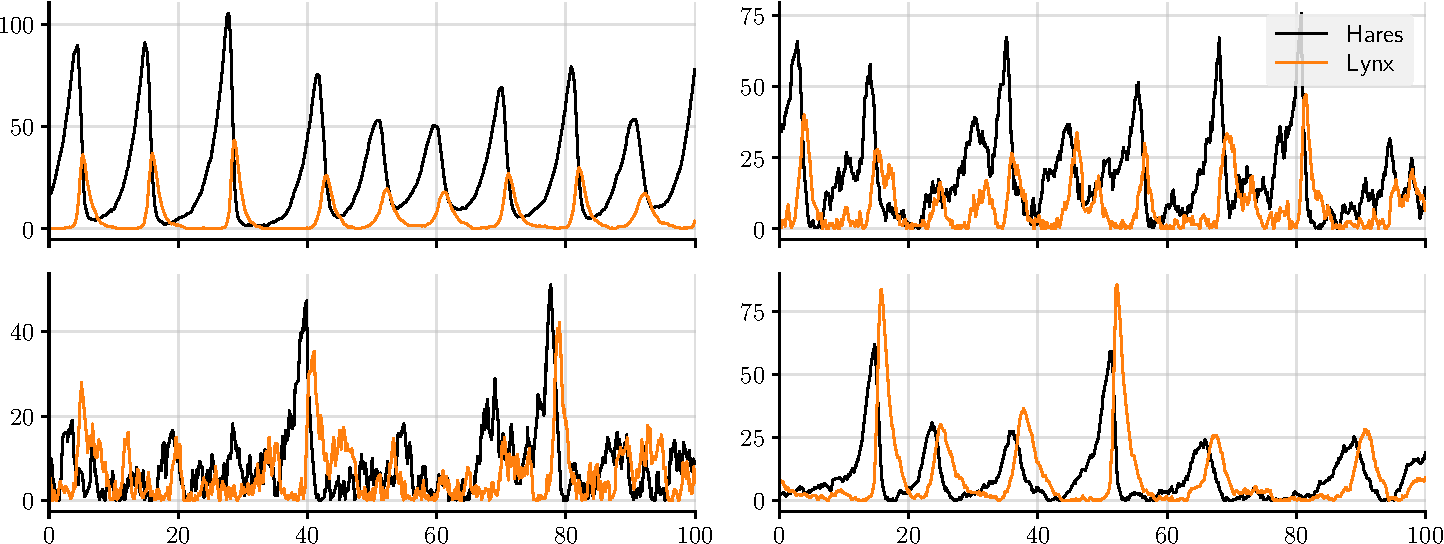
\includegraphics[width=\linewidth]{\gp{experiments/predprey_simulator/simulation.pdf}}
        \caption{
            Four samples from the proposed stochastic version of the Lotka--Volterra equations \eqref{eq:stoch_Lotka-Volterra_prey} and \eqref{eq:stoch_Lotka-Volterra_predator}.
            The parameters of \eqref{eq:stoch_Lotka-Volterra_prey} and \eqref{eq:stoch_Lotka-Volterra_predator} are sampled according to
             \cref{tab:stoch_Lotka-Volterra_parameters}.
        }
        \label{fig:samples_pred-prey_simulator}
    \end{subfigure}
    \caption{
        Hare--lynx data set and proposed stochastic simulator
    }
\end{figure}

Our goal will be to make predictions for the famous hare--lynx data set.
The hare--lynx data set is a time series from 1845 to 1935 recording yearly population counts of a population of Snowshoe hares and a population of Canadian lynx \parencite{MacLulich:1937:Fluctuations_in_the_Numbers_of_the_Varying_Hare}.
A digital version extracted from the original graph by \textcite{MacLulich:1937:Fluctuations_in_the_Numbers_of_the_Varying_Hare}
is available at \url{http://people.whitman.edu/~hundledr/courses/M250F03/LynxHare.txt} \parencite{Hundley:2022:Introduction_to_Mathematical_Modelling}.
\Textcite{Hundley:2022:Introduction_to_Mathematical_Modelling},
the author of this digital source,
says that other authors caution that the hare--lynx data is actually a composition of multiple time series, and presents the data with that caution.
We, therefore, also present the data with this caution.
\Cref{fig:hare-lyxn_data} visualises the hare--lynx data set.

\begin{table}[t]
    \centering
    \caption[
        Parameters of the stochastic Lotka--Volterra equations
    ]
    {
        Sampling distributions for the parameters of the stochastic version of the Lotka--Volterra equations \eqref{eq:stoch_Lotka-Volterra_prey} and \eqref{eq:stoch_Lotka-Volterra_predator}.
        These equations are simulated on a dense grid spanning $[-10, 100]$.
        The table also shows the distribution for the initial conditions at $t = -10$.
        To not depend too heavily on these initial conditions, the simulation results on $[-10, 0]$ are discarded.
    }
    \label{tab:stoch_Lotka-Volterra_parameters}
    \small
    \begin{tabular}{ll}
        \toprule
        Parameter & Distribution \\ \midrule
        Initial condition $X_{-10}$ & $\Unif([5, 100])$ \\ 
        Initial condition $Y_{-10}$ & $\Unif([5, 100])$ \\
        $\alpha$ & $\Unif([0.2, 0.8])$ \\
        $\beta$ & $\Unif([0.04, 0.08])$ \\
        $\gamma$ & $\Unif([0.8, 1.2])$ \\
        $\delta$ & $\Unif([0.04, 0.08])$ \\
        $\nu$ & Fixed to $1/6$ \\
        $\sigma$ & $\Unif([0.5, 10])$ \\
        \bottomrule
    \end{tabular}
\end{table}

To make predictions for the hare--lynx data set, we will use the Lotka--Volterra equations
\parencite{Lotka:1910:Contribution_to_the_Theory_of,Volterra:1926:Variazioni_e_Fluttuazioni_del_Bumero},
also called the predator--prey equations.
The Lotka--Volterra equations are an idealised mathematical model for the population counts of a prey population and a predator population:\index{Lotka--Volterra equations}
\begin{align}
    \hspace{-4cm}\text{prey population:}\qquad
    & x'(t) = \hspace{6.5pt}\alpha x(t) - \beta x(t) y(t), \\
    \hspace{-4cm}\text{predator population:}\qquad
    & y'(t) = -\delta y(t) + \gamma x(t) y(t). 
\end{align}
These differential equations say that the prey population naturally grows exponentially with rate $\alpha$,
and
that the predator population naturally decays exponentially with rate $\delta$.
In addition, the predators hunt the prey.
The resulting additional growth in the predator population
and
the resulting additional decrease in the prey population
are both proportional to the product of the densities.
In this idealised mathematical form, the population counts converge to a smooth, noiseless limit cycle and then perfectly track this limit cycle ever after.
This is unlike real-world predator--prey population counts, which exhibit noisy behaviour and imperfect cycles.
We therefore consider a stochastic version of the Lotka--Volterra equations, given by the following two coupled stochastic differential equations:
\begin{align}
    \label{eq:stoch_Lotka-Volterra_prey}
    \sd X_t &= \hspace{8pt}\alpha X_t \isd t - \beta Y_t X_t \isd t + \sigma X^\nu_t \isd W^{(1)}_t, \\
    \label{eq:stoch_Lotka-Volterra_predator}
    \sd Y_t &= -\gamma X_t \isd t + \delta Y_t X_t \isd t + \sigma Y^\nu_t \isd W^{(2)}_t
\end{align}
where $W^{(1)}$ and $W^{(2)}$ are two independent Brownian motions.
Compared to the Lotka--Volterra equations, \eqref{eq:stoch_Lotka-Volterra_prey} and \eqref{eq:stoch_Lotka-Volterra_predator} have two additional terms, $\sigma X^\nu_t \isd W^{(1)}_t$ and $\sigma Y^\nu_t \isd W^{(2)}_t$, which introduce noisy behaviour.
In these terms, multiplying by $X^\nu_t$ and $Y^\nu_t$ makes the noise go to zero when $X_t$ and $Y_t$ become small, ensuring that $X_t$ and $Y_t$ remain positive.
In addition,
we multiply by a parameter $\sigma > 0$ to control the magnitude of the noise,
and we raise $X_t$ and $Y_t$ to a power $\nu > 0$ to control how quickly the noise grows as $X_t$ and $Y_t$ grow.
Namely, $X_t$ naturally grows exponentially, so, by adding noise of magnitude proportional to $X_t$, we risk large spikes in the prey population.
To moderate this behaviour, we choose $\nu$ to be strictly less than one.
In particular, after simulating from \eqref{eq:stoch_Lotka-Volterra_prey} and \eqref{eq:stoch_Lotka-Volterra_predator} a few times, we settle on $\nu = \tfrac16$. 
\looseness=-1
For the remainder of the parameters, we simply manually play around with
\eqref{eq:stoch_Lotka-Volterra_prey} and \eqref{eq:stoch_Lotka-Volterra_predator}, settle on parameter ranges that look reasonable,
and randomly sample parameters from those intervals.
\Cref{tab:stoch_Lotka-Volterra_parameters} summarises the sampling distributions for all parameters of \eqref{eq:stoch_Lotka-Volterra_prey} and \eqref{eq:stoch_Lotka-Volterra_predator}. 
\Cref{fig:samples_pred-prey_simulator} shows four samples from the proposed stochastic model.

We have constructed a simulator that can generate data which looks roughly like the hare--lynx data.
Following the sim-to-real paradigm, we will generate a meta--data set with this simulator, train a neural process on the meta--data set, and finally apply the neural process to the real hare--lynx data.

To generate a meta--data set,
we simulate \eqref{eq:stoch_Lotka-Volterra_prey} and \eqref{eq:stoch_Lotka-Volterra_predator} on a dense grid spanning 110 years, throw away the first 10 years, and retain between 150 and 250 data points for $X_t$ and $Y_t$.
The numbers of data points and the locations of the data points are sampled separately for $X_t$ and $Y_t$.
Hence, whereas the hare--lynx data is regularly spaced and the populations are always simultaneously observed, our simulator generates data at arbitrary and nonsimultaneous points in time.
We split these data sets into context and target sets in three different ways.
First, for $X_t$ and $Y_t$ separately, randomly designate 100 points to be the target points and let the remainder be the context points.
This task is called \emph{interpolation} and is the primary measure of performance.
Second, select a random time between 25 years and 75 years, let everything before that time be the context set, and let everything after that time be the target set.
This task is called \emph{forecasting} and measures the model's ability extrapolate the cyclic behaviour.
Third, randomly choose $X_t$ or $Y_t$ and, for the choice, split the data in two exactly like for forecasting.
For $X_t$ or $Y_t$ that was not chosen, append all data to the context set.
This task is called \emph{reconstruction} and measures the model's ability to infer one population count from the other.
To train the models, for every batch, we randomly choose one of these tasks by rolling a three-sided die.
We will also perform these tasks on the real hare--lynx data;
in that case, for interpolation, we let the number of target points per output be between one and fifteen.
The tasks on simulated and real data are similar, but slightly differ in the number of context and target points.

We compare the strongest newly proposed models against the strongest existing baselines.
Based on \cref{sec:experiments:synthetic}, we choose to compare the ConvCNP, ConvGNP, FullConvGNP, and AR ConvCNP against the ACNP, ANP, ConvNP, and AR ACNP.
\looseness=-1
To deal with the positivity of population counts, we transform the marginals of all models to distributions on $(0, \infty)$ by pushing the marginals through $x \mapsto \log(1 + x)$.
\Cref{\xrprefix{sec:experimental_details:models}} describes the general architectures of the models, \cref{\xrprefix{sec:experimental_details:protocols}} describes the general training, cross-validation, and evaluation protocols, and \cref{\xrprefix{sec:experimental_details:predprey}} describes details specific to this experiment.

\begin{table}[t]
    \centering
    \caption[
        Results for the predator--prey experiments
    ]{
        Normalised log-likelihoods in the predator--prey experiments.
        Shows the performance for
        interpolation (``Int.''),
        forecasting (``For.''),
        and reconstruction (``Rec.'')
        on simulated (``S'')
        and real (``R'') data.
        Models are ordered by interpolation performance on simulated data.
        See \cref{sec:experiments:predprey} for a more detailed description.
        \latentvariabledescription
        \numbersdescription
    }
    \label{tab:predprey_results}
    \small
    \setlength{\tabcolsep}{1.5pt}
    \subimport{tables/}{predprey_results.tex}
\end{table}

\begin{figure}[t]
    \centering
    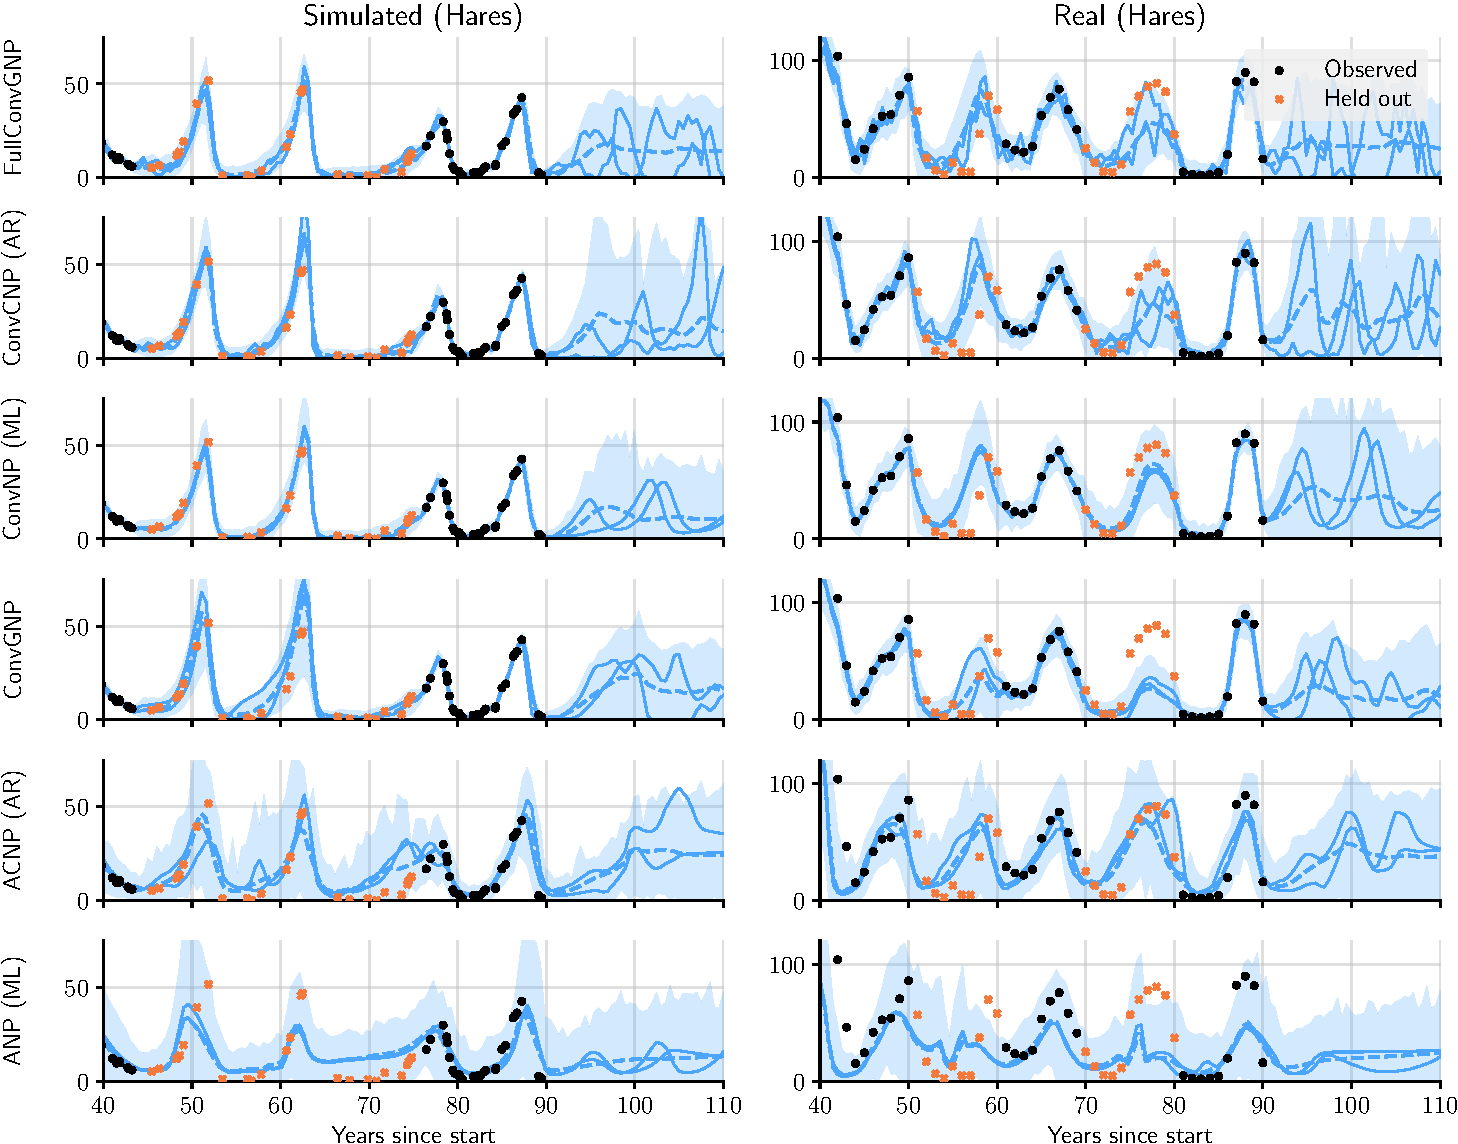
\includegraphics[width=\linewidth]{\gp{experiments/predprey_predictions/predictions.pdf}}
    \caption[
        Predictions by the best performing models in the predator--prey experiment
    ]{
        Predictions by the best performing models in the predator--prey experiment.
        \emph
        Shows predictions for data generated from the simulator (left) and predictions for the real hare--lynx data (right).
        The models observe all lynx population counts and some hare population counts.
        The plots show predictions for some observed and some unobserved hare population counts.
        Filled regions are central 95\%-credible regions.
    }
    \label{fig:predprey_predictions}
    \vspace*{-0.5em}
\end{figure}


\paragraph{Results}
For simulated data,
\Cref{tab:predprey_results} shows the results for interpolation, forecasting, and reconstruction, and
the left column of \cref{fig:predprey_predictions} illustrates predictions by the models.
The FullConvGNP and AR ConvCNP take a shared top position in the results.
For interpolation, the ConvNP, ConvGNP, and ConvCNP come a close second;
and for reconstruction, the AR ConvCNP outperforms the FullConvGNP.
Note that, for interpolation, the ConvGNP fails to outperform the ConvCNP,
which indicates that ConvGNP was unable to successfully exploit dependencies between target outputs in this task.
Also note that the AR ConvCNP outperforms the ConvCNP, ConvGNP, and the ConvNP;
and that the AR ACNP outperforms the ACNP and the ANP.
This again demonstrates that running CNPs in AR mode can improve performance and can even outperform strong GNPs and LNPs.

After having the trained and evaluated the models on data generated with our stochastic version of the Lotka--Volterra equations, we finally apply the models to the real hare--lynx data set.
\Cref{tab:predprey_results} again shows the results for all three tasks,
and the right column of \cref{fig:predprey_predictions} illustrates predictions by the models.
Whereas the FullConvGNP shared the top position with the AR ConvCNP for the simulated data,
the FullConvGNP now shares the top position with the AR ACNP and ANP.
For the simulated data in \cref{fig:predprey_predictions}, predictions appear appropriately calibrated.
For the real hare--lynx data in \cref{fig:predprey_predictions}, however, the predicted uncertainties look much less well calibrated,
and sometimes even fail to capture the data.
We conclude that the neural processes trained on our simulator can be used to produce acceptable predictions.
However, these predictions are not perfectly calibrated,
so we also conclude that there is a statistical mismatch between the simulator and the real hare--lynx data.
\looseness=-1
That there is a statistical mismatch is corroborated by the observation
 that the log-likelihoods for the real data are generally much lower than for the simulated data.

To alleviate accidental overconfidence due to mismatch between the simulator and the real data,
it works in a model's favour to generally produce predictions with bigger uncertainty.
\Cref{fig:predprey_predictions} shows that the convolutional models tightly fit the simulated data,
whereas the AR ACNP and ANP generally produce bigger uncertainties.
Consequently, the convolutional model comparably perform worse on the real data,
and the AR ACNP and ANP comparably perform better.

\section{Electroencephalography Experiments}
\label{sec:experiments:eeg}

\begin{figure}[t]
    \centering
    \small
    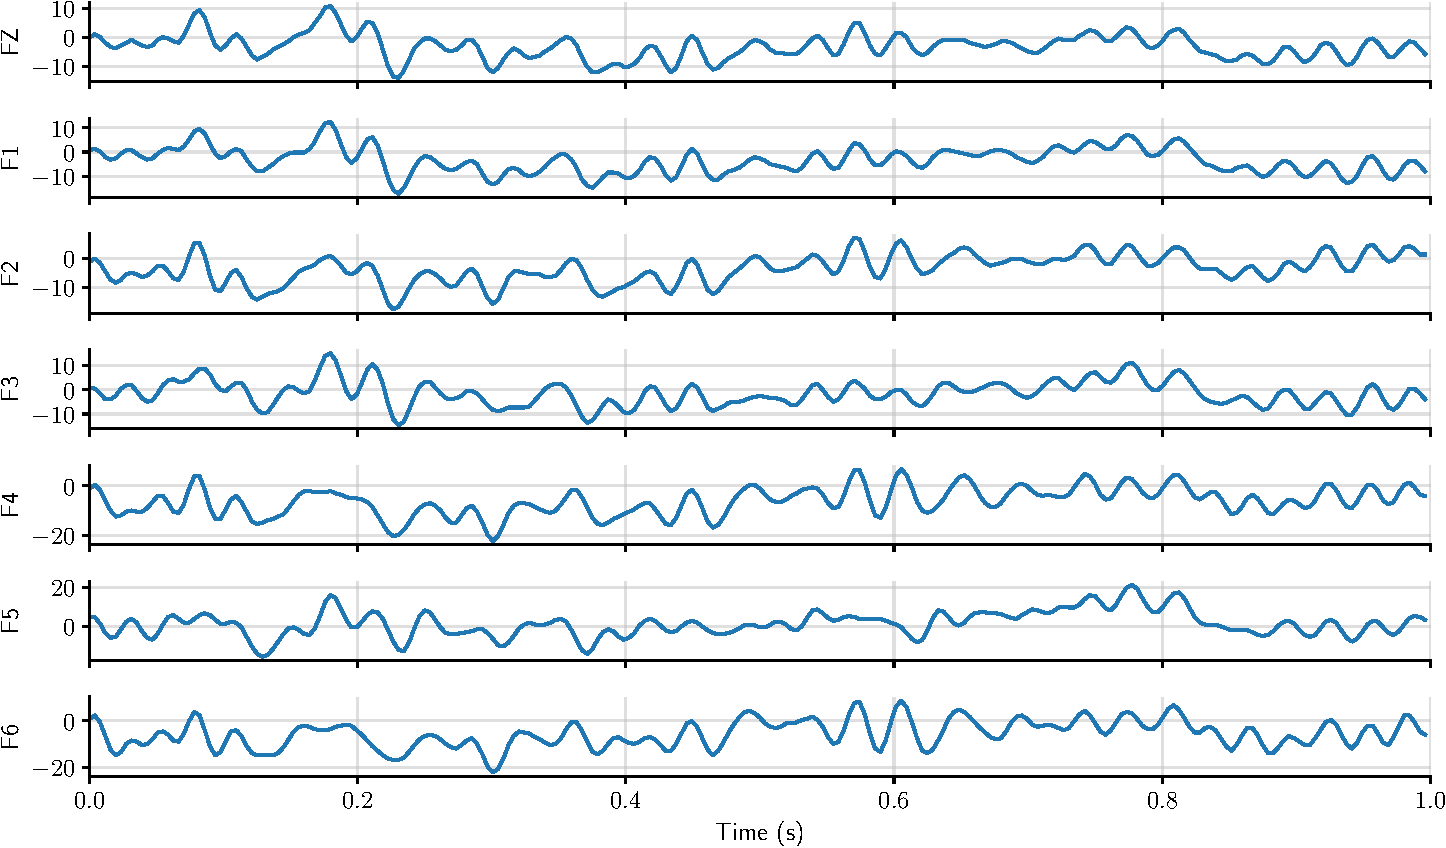
\includegraphics[width=\linewidth]{\gp{experiments/eeg_data/example.pdf}}
    \caption[
        Example of trial in the EEG data set
    ]{
        Example of trial in the EEG data set.
        Note that the signals for all electrodes appear correlated, but are subtly different. 
    }
    \label{fig:eeg_example}
\end{figure}

In the third experiment, 
we explore an electroencephalography data set collected from 122 subjects
\parencite{Begleiter:2022:EEG_Database_Data_Set}.
There are two groups of subjects: alcoholic and control.
Every subject was subjected to a single stimulus or two stimuli,
and their response was measured with 64 electrodes placed on a subject's scalp.
These measurements are in terms of \emph{trials}, where a trial consists of 256 samples of the electrodes spanning one second.
The data sets contains up to 120 trials for each subject.
The data is available at \url{https://archive.ics.uci.edu/ml/datasets/eeg+database}
and the collection is described in detail by \textcite{Zhang:1995:Event_Related_Potentials_During_Object}.
\looseness=-1
In this experiment, we focus only on seven frontal electrodes: FZ, F1, F2, F3, F4, F5, and F6.
\Cref{fig:eeg_example} illustrates a trial of a subject, showing the samples for these seven electrodes.

\begin{table}[t]
    \centering
    \caption[
        Results for the EEG experiments
    ]{
        Normalised log-likelihoods in the EEG experiments.
        Shows the performance for
        interpolation,
        forecasting,
        and reconstruction.
        Models are ordered by interpolation performance.
        See \cref{sec:experiments:eeg} for a more detailed description.
        \latentvariabledescription
        \numbersdescription
    }
    \label{tab:eeg_results}
    \small
    \subimport{tables/}{eeg_results.tex}
\end{table}

\begin{figure}[t]
    \centering
    \small
    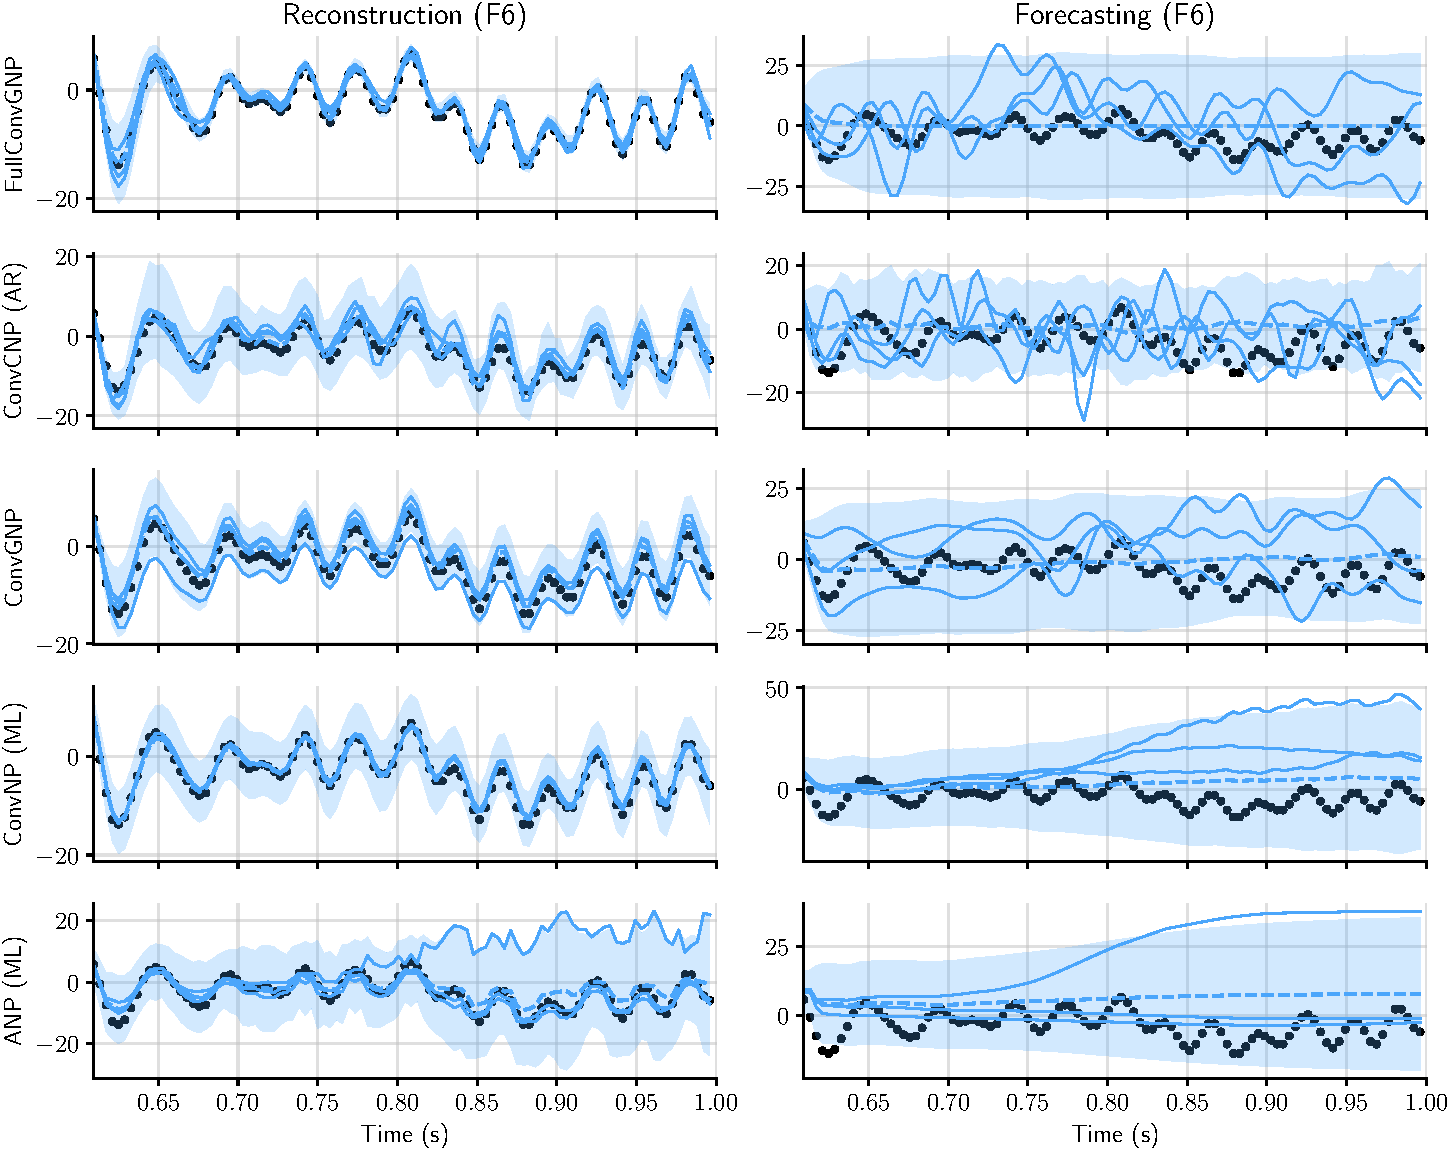
\includegraphics[width=\linewidth]{\gp{experiments/eeg_prediction/prediction.pdf}}
    \caption[
        Predictions by the best performing models in the EEG experiment
    ]
    {
        Predictions by the best performing models in the EEG experiment.
        The data in this example experiment is the sample trial from \cref{fig:eeg_example}.
        In both tasks, the models predict the last 100 samples of electrode F6.
        In the reconstruction task, the models observe for electrodes FZ and F1--F5 the entire signal and for electrode F6 only the first 156 samples.
        In the forecasting task, the models observe for all electrodes only the first 156 samples.
        Filled regions are central 95\%-credible regions.
    }
    \label{fig:eeg_prediction}
\end{figure}

We randomly split all subjects into three sets:
an evaluation set consisting of ten subjects,
a cross-validation set consisting of ten other subjects,
and a training set consisting of all remaining subjects.
For each of these sets, we create a meta--data set by aggregating the trials for all subjects.
We split every trial into a context and target set in the same three ways as for the predator--prey experiment (\cref{sec:experiments:predprey}).
First, for all seven electrodes separately, randomly designate between 50 and 100 points to be the target points and let the remainder be the context points.
This task is called \emph{interpolation} and is the primary measure of performance.
Second, select a random time between \SI{0.5}{s} and \SI{0.75}{s}, let everything before that time be the context set, and let everything after that time be the target set.
This task is called \emph{forecasting} and measures the model's ability extrapolate.
Third, randomly choose one of the seven electrodes and, for that choice, split the data in two exactly like for forecasting.
For all other electrodes, append all data to the context set.
\looseness=-1
This task is called \emph{reconstruction} and measures the model's ability to infer a signal for one electrode from the others.
To train the models, for every batch, we randomly choose one of the tasks by flipping a three-sided coin.

Like for the predator--prey experiment (\cref{sec:experiments:predprey}), we compare the ConvCNP, ConvGNP, FullConvGNP, and AR ConvCNP against the ACNP, ANP, ConvNP, and AR ACNP.
\Cref{\xrprefix{sec:experimental_details:models}} describes the general architectures of the models, \cref{\xrprefix{sec:experimental_details:protocols}} describes the general training, cross-validation, and evaluation protocols, and \cref{\xrprefix{sec:experimental_details:eeg}} describes details specific to this experiment.
We remark that architecture of the ANP required modifications in order to scale the model,
and that the training of the FullConvGNP and ANP were cut short after having run for 45 hours;
see \cref{\xrprefix{sec:experimental_details:eeg}} for more details.

\paragraph{Results}
\Cref{tab:eeg_results} presents the results for interpolation, forecasting, and reconstruction,
and \cref{fig:eeg_prediction} illustrates predictions by the models.
On all three tasks, the FullConvGNP outperforms all other models.
For interpolation, the AR ConvCNP comes second;
and, for forecasting, the ConvGNP is a close second.
For reconstruction, however, no other model comes close.
Note that the AR ConvCNP outperforms the ConvGNP in the interpolation and reconstruction tasks,
but the ConvGNP performs substantially better in the forecasting task.
This is a rather strong performance by the ConvGNP.
Except for the ConvGNP, for strictly all models, the forecasting and reconstruction log-likelihoods are worse than the interpolation log-likelihood.
For the ConvGNP, the forecasting log-likelihood is best and considerably improves over the interpolation log-likelihood.
This strong performance of the ConvGNP is confirmed by \cref{fig:eeg_prediction}, where the prediction of the ConvGNP in the forecasting task is indeed similar to that of the FullConvGNP.

\section{Climate Downscaling}
\label{sec:experiments:climate}

\index{downscaling}
In the last experiment, we explore a climate science application.
In climate modelling, future projections are generated by integrating the atmospheric equations of motion forward in time using a numerical solver.
Unfortunately, computational constraints typically limit the spatial resolution of those projections to around \SI{100}{km} \parencite{Eyring:2016:Overview_of_the_Coupled_Model},
which is insufficient to resolve extreme events and produce local predictions \parencite{Stocker:2013:Climate_Change_2013,Maraun:2017:Towards_Process-Informed_Bias_Correction_of}.
Statistical downscaling methods attempt to address this issue by refining the coarse-grained outputs
into more fine-grained predictions
\parencite{Maraun:2018:Statistical_Downscaling_and_Bias_Correction}.
While numerous data-driven approaches exist,
statistical downscaling methods are often limited to making predictions at a fixed set of points at which historical observations are available 
\parencite{
Vandal:2017:DeepSD_Generating_High_Resolution_Climate,
Bhardwaj:2018:Downscaling_Future_Climate_Change_Projections,
Misra:2018:Statistical_Downscaling_of_Precipitation_Using,
Sachindra:2018:Statistical_Downscaling_of_Precipitation_Using,
Vandal:2018:Quantifying_Uncertainty_in_Discrete-Continuous_and,
Vandal:2019:Intercomparison_of_Machine_Learning_Methods,
Pan:2019:Improving_Precipitation_Estimation_Using_Convolutional,
Singh:2019:Downscaling_Numerical_Weather_Models_with_GANs,
Bano-Medina:2020:Configuration_and_Intercomparison_of_Deep,
Liu:2020:Climate_Downscaling_Using_YNet_A}.

Recently, \textcite{Vaughan:2022:Convolutional_Conditional_Neural_Processes_for} used the ConvCNP to perform statistical downscaling.
Compared to existing downscaling methods, a notable feature of the ConvCNP is that the model is not limited to a fixed set of points, but can make fine-grained predictions anywhere.
However, as we discussed in \cref{\xrprefix{sec:convcnps:gnp}}, the ConvCNP does not model dependencies between target outputs, and is consequently unable to produce coherent samples.
This limits the applicability of \citeauthor{Vaughan:2022:Convolutional_Conditional_Neural_Processes_for}'s approach,
because the ability to model dependencies is important for downstream applications.
For example, to estimate the maximum temperature of a region, as opposed to single point location, it is necessary to model spatial dependencies.
In this experiment,
we extend \citeauthor{Vaughan:2022:Convolutional_Conditional_Neural_Processes_for}'s
approach to the ConvGNP and AR ConvCNP.
Importantly,
the ConvGNP and AR ConvCNP model spatial dependencies,
so we broaden the downstream applicability of \citeauthor{Vaughan:2022:Convolutional_Conditional_Neural_Processes_for}'s approach.

Thus far, context sets and target sets have consisted of data from the same domain.
Specifically, in \cref{\xrprefix{sec:predmap:motivation}},
we proposed a motivating generative model where
the context and target set both consist of noisy observations of the same ground-truth stochastic process $f$.
However,
nowhere in our developments have we actually used or required that the outputs of the context and target sets live in the same space!
In fact, all models that we have considered so far also work when the outputs of the context sets are vectors of a different dimensionality than the outputs of the target set.
In the CNP (\cref{\xrprefix{mod:cnp}}) and GNP (\cref{\xrprefix{mod:gnp}}), this simply means that the MLP $\phi_\theta$ of the encoder takes in more of fewer $y$-dimensions;
and in the ConvCNP (\cref{\xrprefix{mod:convcnp}}), ConvGNP (\cref{\xrprefix{mod:convgnp}}), and FullConvGNP (\cref{\xrprefix{mod:fullconvgnp}}), this simply means that the CNN takes in more or fewer data channels---no other modifications are necessary.
This generalisation might not have been immediately apparent earlier, because we only considered one-dimensional outputs for notational simplicity.
Letting the outputs of the context and target sets be from different domains says, very simply, to make predictions for \emph{some data} based on \emph{other data}.\footnote{
    For translation equivariance (\cref{\xrprefix{def:translation_equivariance}}) to make sense,
    we do require that the inputs of the context and target set live in the same space.
    However, should we not be concerned with translation equivariance,
    then the inputs need not live in the same space either.
}
In a way, this formulation is even simpler than what we have considered so far.
\citeauthor{Vaughan:2022:Convolutional_Conditional_Neural_Processes_for}'s
(\citeyearlabel{Vaughan:2022:Convolutional_Conditional_Neural_Processes_for})
approach is based on this interpretation of neural processes.
\looseness=-1
Before we explain the setup of the ConvCNP and the extension to the ConvGNP and AR ConvCNP, we first detail the experimental setup.

\begin{figure}[t]
    \centering
    \small
    \begin{subfigure}[t]{0.48\linewidth}
        \centering
        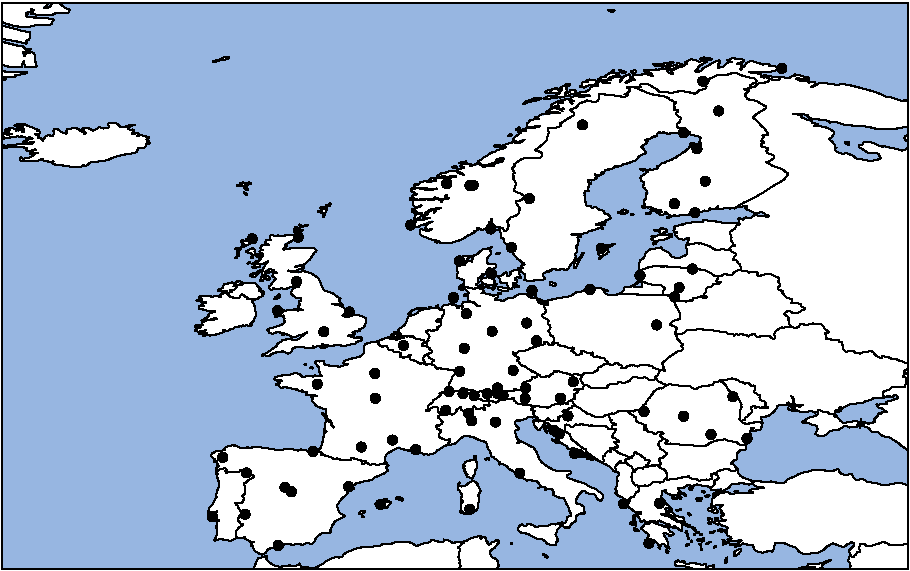
\includegraphics[height=4.5cm]{\gp{experiments/climate_station_locations/value_locations.pdf}}
        \caption{
            VALUE: 86 weather stations
        }
        \label{fig:locations_value}
    \end{subfigure}
    \hfill
    \begin{subfigure}[t]{0.48\linewidth}
        \centering
        \includegraphics[height=4.5cm]{\gp{experiments/climate_station_locations/germany_locations.pdf}}
        \caption{
            Germany: 589 weather stations 
        }
        \label{fig:locations_germany}
    \end{subfigure}
    \caption[
        Locations of weather stations in climate downscaling and fusion experiments
    ]
    {
        Locations of the weather stations in the VALUE and Germany downscaling and fusion experiments
    }
\end{figure}


In this experiment, we will consider two statistical downscaling tasks:
the \emph{VALUE task} and the \emph{Germany task}.
The VALUE task follows the VALUE framework \parencite{Maraun:2015:VALUE_A_Framework_to_Validate}, which provides results for a large ensemble of frequently used downscaling methods on a standardised set of tasks.
More specifically, for the VALUE task, we consider experiment 1a from the VALUE framework
and estimate the maximum daily temperature at 86 weather stations around Europe.
To estimate these temperatures, we follow \textcite{Vaughan:2022:Convolutional_Conditional_Neural_Processes_for} and use 25 coarse-grained ERA-Interim reanalysis variables \parencite{Dee:2011:The_ERA-Interim_Reanalysis_Configuration_and} in combination with \SI{1}{km}--resolution elevation data \parencite{EROSC:1997:GPTOTO30}.
We consider the following 25 ERA-Interim reanalysis variables:
\begin{itemize}
    \item at the surface: maximum temperature, mean temperature, northward wind, and eastward wind;
    \item in the upper atmosphere at \SI{850}{hPa}, \SI{700}{hPa}, and \SI{500}{hPa}: specific humidity, temperature, northward wind, and eastward wind; and
    \item
        invariant features:
        angle of sub-grid-scale orography,
        anisotropy of sub-grid-scale orography,
        standard deviation of filtered sub-grid-scale orography,
        standard deviation of orography,
        geopotential,
        longitude,
        latitude, and
        fractional position in the year $t$ transformed encoded with $t \mapsto (\cos(2\pi t), \sin(2 \pi t))$.
\end{itemize}
These variables are bilinearly interpolated to a $2^\circ$-resolution grid.
The temperature data is provided by the VALUE framework at \url{http://www.value-cost.eu/data} and the ERA-Interim reanalysis data is available at \url{https://www.ecmwf.int/en/forecasts/datasets/reanalysis-datasets/era-interim}.
The \SI{1}{km}--resolution elevation data is available at
\url{https://doi.org/10.5066/F7DF6PQS}.
The locations of the weather stations around Europe are visualised in \cref{fig:locations_value}.

For the Germany task, we estimate the maximum daily temperature at 589 weather stations around Germany using the same 25 coarse-grained ERA-Interim reanalysis variables and the same \SI{1}{km}--resolution elevation data.
In this case, however, the ERA-Interim reanalysis variables are used at their native 0.75$^\circ$-resolution grid.
The weather station data are a subselection of the European Climate Assessment \& Dataset \parencite{Klein_Tank:2002:Daily_Dataset_of_20th-Century_Surface} and are available at \url{https://www.ecad.eu};
we use the blended data.
The locations of the weather stations around Germany are visualised in \cref{fig:locations_germany}.

\paragraph{Part 1: downscaling with the MLP ConvCNP and MLP ConvGNP}
This experiment consists of two parts.
In this first part, we perform the VALUE and Germany downscaling tasks by setting up the context and target sets as follows.
For every day,
let the context set be the 25 coarse-grained ERA-Interim reanalysis variables
and let the target set be the observations of the weather stations---we will shortly explain how the \SI{1}{km}--resolution elevation data is incorporated.
As we previously explained, there is no problem in letting the context and target data be from different domains.
For the ConvCNP and ConvGNP, we set the internal discretisation (\cref{\xrprefix{proc:discretisation}}) equal to the $2^\circ$ or $0.75^\circ$-resolution grid of the ERA-Interim reanalysis variables.
Moreover, following \textcite{Vaughan:2022:Convolutional_Conditional_Neural_Processes_for}, rather than using a U-Net architecture, we use a residual convolutional neural network  \parencite{He:2016:Deep_Residual_Learning_for_Image} with depthwise-separable convolutions \parencite{Chollet:2017:Xception_Deep_Learning_With_Depthwise}.
To incorporate the \SI{1}{km}--resolution elevation data, one approach would be to also include this data in the context set.
However, we would then have to increase the resolution of the discretisation from $2^\circ$ or $0.75^\circ$ to \SI{1}{km}; 
otherwise, much of the detail in the elevation data would be lost.
Unfortunately, making the discretisation this much finer would come with a substantial increase in computational cost.
Instead, \citeauthor{Vaughan:2022:Convolutional_Conditional_Neural_Processes_for} propose a different approach.
After the CNN architecture, insert a pointwise multilayer perceptron (MLP) which, at every target input, fuses the local elevation with the output of the CNN architecture:

\index{pointwise MLP}
\begin{definition}[Pointwise MLP; \theoremcite{Vaughan:2022:Convolutional_Conditional_Neural_Processes_for}]
    \label{def:pointwise_MLP}
    Consider a neural process with a decoder $\dec_\theta$ operating on a functional encoding (\cref{\xrprefix{def:functional_encoding}}):
    $
        \dec_\theta \colon C(\X, \R^{K_1}) \to C(\X, \R^{K_2}).
    $
    Let $\mathsf{aux}\colon \X \to \R^{K_3}$ be auxiliary information.
    We say that the neural process \emph{incorporates the auxiliary information with a pointwise MLP} if the decoder is of the form $\dec_\theta = \mathsf{fuse}_\theta \comp \dec'_\theta$ where
    $\dec'_\theta\colon C(\X, \R^{K_1}) \to C(\X, \R^{\widetilde K_2})$ and
    \begin{align}
        \mathsf{fuse}_\theta &\colon C(\X, \R^{\widetilde K_2}) \to C(\X, \R^{K_2}), \quad
        \mathsf{fuse}_\theta(\vz(\vardot)) = \mathsf{MLP}_\theta(\vz(\vardot), \mathsf{aux}(\vardot))
    \end{align}
    with $\mathsf{MLP}_\theta \colon \R^{\widetilde K_2 + K_3} \to \R^{K_2}$ a multi-layer perceptron called the \emph{pointwise MLP}.
\end{definition}

\index{ConvCNP!MLP}
\index{ConvGNP!MLP}
We let the ConvCNP and ConvGNP incorporate the \SI{1}{km}--resolution elevation data using a pointwise MLP in the sense of \cref{def:pointwise_MLP};
specifically, $\mathsf{aux}$ produces the elevation at any input using bilinear interpolation.
We call these variations of the ConvCNP and ConvGNP the \emph{MLP ConvCNP} and \emph{MLP ConvGNP} respectively.

\begin{table}[t]
    \centering
    \caption[
        Results for the climate downscaling experiments
    ]{
        Normalised log-likelihoods and mean absolute errors (MAEs) in the climate downscaling experiments.
        Shows the performance on the VALUE and Germany downscaling tasks averaged over the five folds from the VALUE protocol \parencite{Maraun:2015:VALUE_A_Framework_to_Validate}.
        The MAE is the mean of the MAE per station.
        The MAE of the VALUE models are computed from results published at \url{http://www.value-cost.eu/validationportal}.
        VALUE models refer to the models used the comparison of 52 downscaling approaches \parencite[\url{http://www.value-cost.eu};][]{Maraun:2015:VALUE_A_Framework_to_Validate,Gutirrez:2019:An_Intercomparison_of_a_Large}.
        ``PP'' stands for perfect prognosis and refers to the class of VALUE models which are comparable to the models in this chapter \parencite{Maraun:2010:Precipitation_Downscaling_Under_Climate_Change}.
        Errors indicate the central 95\%-confidence interval.
        Numbers which are significantly best ($p < 0.05$) are boldfaced.
    }
    \label{tab:climate_downscaling_results}
    \small
    % Mean of stationwise MAE:
    \begin{tabular}{lcccc}
        \toprule
        \multirow{2}{*}{Model} & VALUE & & Germany &  \\
                               & Log-lik. & MAE & Log-lik.~\hspace{2pt} & MAE \\
        \midrule
        ConvCNP (MLP)
            & $\shortminus 1.66 \, {\scriptstyle \pm 0.00}$
            & $\mathbf{1.04} \, {\scriptstyle \pm 0.04}$
            & $\shortminus 1.62 \, {\scriptstyle \pm 0.01}$
            & $\mathbf{1.00} \, {\scriptstyle \pm 0.05}$ \\
        ConvGNP (MLP)
            & $\mathbf{\shortminus 1.63} \, {\scriptstyle \pm 0.00}$
            & $\mathbf{1.01} \, {\scriptstyle \pm 0.04}$
            & $\mathbf{\shortminus 1.45} \, {\scriptstyle \pm 0.00}$
            & $1.14 \, {\scriptstyle \pm 0.06}$ \\
        Best VALUE PP model
            &
            & $1.37 \, {\scriptstyle \pm 0.05}$ \\
        Best VALUE model
            &
            & $1.20 \, {\scriptstyle \pm 0.08}$ \\
        \bottomrule
    \end{tabular}
\end{table}

We perform the VALUE and Germany downscaling tasks for all days of the years 1979--2008.
Following the VALUE framework \parencite{Maraun:2015:VALUE_A_Framework_to_Validate}, we split these years into five folds.
On each of the five folds, we evaluate the neural process, using the four other folds for training and holding out the last 1000 days of the training folds for cross-validation.
\Cref{\xrprefix{sec:experimental_details:protocols}} describes the general training, cross-validation, and evaluation protocols, and
\Cref{\xrprefix{sec:experimental_details:climate}} describes the architectures and further details specific to this experiment. 

\paragraph{Results}
The VALUE framework includes results for 52 downscaling approaches \parencite[\url{http://www.value-cost.eu/};][]{Maraun:2015:VALUE_A_Framework_to_Validate,Gutirrez:2019:An_Intercomparison_of_a_Large}.
Amongst these 52 approaches,
the category that is comparable to our neural process approach is called \emph{perfect prognosis} (PP) \parencite{Maraun:2010:Precipitation_Downscaling_Under_Climate_Change}.
\Cref{tab:climate_downscaling_results} shows the results of the MLP ConvCNP and MLP ConvGNP on the VALUE and Germany downscaling tasks and compares these results to the overall best and the best PP approach from the VALUE framework.
%
Compared to all 52 downscaling approaches,
the MLP ConvCNP and MLP ConvGNP achieve
24\%--26\% lower MAE than the best comparable PP model and
18\%--20\% lower MAE than the overall best performing approach.
In addition, compared to the ConvCNP MLP, the ConvGNP MLP achieves a moderate but statistically significant improvement in log-likelihood.

\begin{figure}[t]
    \centering
    \small
    \includegraphics[width=\linewidth]{\gp{experiments/climate_convgnp_sample/sample.pdf}}
    \caption[
        Prediction by the MLP ConvGNP in the Germany downscaling experiment
    ]{
        Mean prediction by and two samples from the MLP ConvGNP for an arbitrary day in the Germany downscaling experiment.
        For the samples, shows the difference with respect to the mean.
    }
    \label{fig:climate_convgnp_sample}
\end{figure}


In the VALUE task, most weather stations are geographically far apart,
so daily maximum temperatures at these weather stations are only moderately correlated.
For this reason, the benefits of the ConvGNP MLP over the ConvCNP MLP are less pronounced.
On the other hand, in the Germany task, the weather stations are geographically more nearby, so the daily maximum temperatures in this task are more strongly correlated.
This is reflected in \Cref{tab:climate_downscaling_results}, which shows that, in the Germany task, the MLP ConvGNP gives a bigger improvement in log-likelihood over the MLP ConvCNP than in the VALUE task.
Note, however, that the MAE of the MLP ConvGNP is worse than that of the MLP ConvCNP.
\looseness=-1
This is reasonable, as the MLP ConvGNP must spend model capacity on modelling dependencies, whereas the MLP ConvCNP can fully focus on the marginals.
\Cref{fig:climate_convgnp_sample} illustrates two samples from the MLP ConvGNP over Germany.
The samples exhibit a realistic degree of variability.

\paragraph{Part 2: downscaling and fusion with the AR ConvCNP}
We have demonstrated that the MLP ConvGNP can be used to successfully model dependencies between outputs in a statistical downscaling task, improving log-likelihoods over the MLP ConvCNP (\cref{tab:climate_downscaling_results}) and enabling coherent samples (\cref{fig:climate_convgnp_sample}).
In this second part of this experiment, we demonstrate that the AR ConvCNP can also be used for this purpose.
Deploying the AR ConvCNP in this task, however, comes with a significant challenge.
In the autoregressive sampling procedure (\cref{\xrprefix{proc:ar}}), samples from the model will be fed back into the model.
If samples of the AR ConvCNP are to be of the same level of quality as the MLP ConvGNP and, in particular, are to vary on the same spatial scale, then the AR ConvCNP must handle context data which varies on this spatial scale.
Since the elevation data is on a \SI{1}{km}--resolution grid, samples of the MLP ConvGNP will also vary on roughly this spatial scale.
Consequently, the discretisation of the AR ConvCNP must also be a \SI{1}{km}--resolution grid, and
we previously argued that such a discretisation would be prohitively expensive!
We must therefore innovate on AR ConvCNP design to come up with a convolutional architecture that can handle such a fine discretisation at reasonable computational expense.

\begin{figure}[t]
    \centering
    \begin{tikzpicture}[remember picture]
        \node [align=center] (hr) at (0,0) {
            $\displaystyle
                \vz\ss{hr}(\vardot)
                = \mathsf{CNN}\ss{hr}\parens*{
                    \begin{bmatrix}
                        \tikzmarknode{zmr}{\vz\ss{mr}(\vardot)} \\
                        \mathsf{data}(D\ss{hr}) \\
                        \mathsf{density}(D\ss{hr})
                    \end{bmatrix}
                }
            $
        };
        \node [align=center, anchor=west] (mr) at ($(zmr.west) + (0, 2)$) {
            $\displaystyle
                \hspace{-4pt}\tikzmarknode{zmrstart}{\vz\ss{mr}(\vardot)}
                = \mathsf{CNN}\ss{mr}\parens*{
                    \begin{bmatrix}
                        \tikzmarknode{zlr}{\vz\ss{lr}(\vardot)} \\
                        \mathsf{data}(D\ss{mr}) \\
                        \mathsf{density}(D\ss{mr})
                    \end{bmatrix}
                }
            $
        };
        \draw [line, ->] ([yshift=-2pt]zmrstart.south) -- ([yshift=2pt]zmr.north);
        \node [align=center, anchor=west] (lr) at ($(zlr.west) + (0, 2)$) {
            $\displaystyle
                \hspace{-4pt}\tikzmarknode{zlrstart}{\vz\ss{lr}(\vardot)}
                = \mathsf{CNN}\ss{lr}\parens*{
                    \begin{bmatrix}
                        \mathsf{data}(D\ss{lr}) \\
                        \mathsf{density}(D\ss{lr})
                    \end{bmatrix}
                }
            $
        };
        \draw [line, ->] ([yshift=-2pt]zlrstart.south) -- ([yshift=2pt]zlr.north);
        \node [yshift=-5pt] (zmrmidway) at ($(zmrstart)!0.5!(zmr)$) {};
        \draw [thick, dashed]
            (current bounding box.west |- zmrmidway)
            --
            (current bounding box.east |- zmrmidway)
            node [pos=1, anchor=north east] {\small $0.01^\circ$ (\good), local to target points (\bad)}
        ;
        \node [yshift=-2pt] (zlrmidway) at ($(zlrstart)!0.5!(zlr)$) {};
        \draw [thick, dashed]
            (current bounding box.west |- zlrmidway)
            --
            (current bounding box.east |- zlrmidway)
            node [pos=0, anchor=south west, yshift=45pt] {\small $\tikzmarknode{res}{0.75^\circ}$ (\bad), \tikzmarknode{where}{covering all of Germany} (\good)}
            node [pos=0, anchor=north west] {\small $0.1^\circ$ (\mediumgood), covering a medium-sized square (\mediumgood)}
        ;
    \draw [line, line width=0.5pt, <-] ([yshift=-2pt]res.south) |- ++(0.35, -0.5) node [anchor=west] {\scriptsize resolution of discretisation};
    \draw [line, line width=0.5pt, <-] (where.north) |- ++(0, 0.3) node [anchor=south] {\scriptsize positioning of discretisation};
    \end{tikzpicture}
    \captionsetup{font=footnotesize}
    \caption[
        Multiscale architecture for the AR ConvCNP
    ]{
        \footnotesize
        Multiscale architecture for the AR ConvCNP.
        A cascade of three convolutional deep sets (\cref{\xrprefix{thm:conv_deep_set}})
        representing a low-resolution, medium-resolution, and high-resolution component.
        Shows the resolution and positioning of the internal discretisation for every convolutional deep set.
        The context set $D = D\ss{lr} \cup D\ss{mr} \cup D\ss{hr}$ is also divided into
        a low-resolution $D\ss{lr}$, medium-resolution $D\ss{mr}$,
        and high-resolution component $D\ss{hr}$.
        The low-resolution context data $D\ss{lr}$ consists of the 25 coarse-grained ERA-Interim reanalysis variables.
        The medium-resolution $D\ss{mr}$ and high-resolution context data $D\ss{hr}$ both consist of the station observations and the \SI{1}{km}--resolution elevation data.
        See \cref{sec:experiments:climate} for more details.
        The functions $\mathsf{data}(D)$ and $\mathsf{density}(D)$ produce respectively the data channel
        and density channel for context data $D$;
        see \cref{\xrprefix{mod:convcnp}} and equations \eqref{\xrprefix{eq:data_channel}} and \eqref{\xrprefix{eq:density_channel}}.
        The maps $\mathsf{CNN}\ss{lr}$, $\mathsf{CNN}\ss{mr}$, and $\mathsf{CNN}\ss{hr}$
        are translation-equivariant maps between functions on $\X$.
        In practice, these maps are all implemented with convolutional neural networks (CNN)
        using the discretisation approach outlined in \cref{\xrprefix{proc:discretisation}}.
        For $\mathsf{CNN}\ss{lr}$, the internal discretisation is the $0.75^\circ$-resolution grid
        corresponding to the 25 coarse-grained ERA-Interim reanalysis variables.
        For $\mathsf{CNN}\ss{mr}$, the internal discretisation is a $0.1^\circ$-resolution grid
        spanning $5^\circ$ more than the most extremal target inputs;
        the discretisation does \emph{not} depend on the context set.
        For $\mathsf{CNN}\ss{hr}$, the internal discretisation is a $0.01^\circ$-resolution grid
        spanning $0.25^\circ$ more than the most extremal target inputs;
        the discretisation also does \emph{not} depend on the context set.
    }
    \label{fig:multires_arch}
\end{figure}

\index{multiscale architecture}
The architecture that we propose is a \emph{multiscale architecture} operating on multiple spatial length scales.
Let us divide the context set $D = D\ss{lr} \cup D\ss{mr} \cup D\ss{hr}$ into
a low-resolution component $D\ss{lr}$, a medium-resolution component $D\ss{mr}$, and a high-resolution component $D\ss{hr}$.
Let the low-resolution component $D\ss{lr}$ consist of features of the context set that vary on a \emph{long} spatial length scale,
the medium-resolution component $D\ss{mr}$ of features that vary on a \emph{medium-range} spatial length scale,
and the high-resolution component $D\ss{hr}$ of features that vary on a \emph{short} spatial length scale. 
The central assumption of the architecture is that predictions for target points depend on precise short-length-scale details $D\ss{hr}$ nearby, but that this dependence weakens as we move away from the target point, starting to depend more on broad-stroke long-length-scale components $D\ss{lr}$.
For example, 
predictions might depend on detailed orographic information nearby,
but more on general orographic shapes farther away.

\Cref{fig:multires_arch} depicts the multiscale architecture.
The architecture is a cascade of three convolutional deep sets, parametrised by three CNNs;
please see the caption.
The low-resolution CNN handles the context data $D\ss{lr}$ with a long spatial length scale.
Because these features have a long spatial length scale, the CNN can get away with a low-resolution discretisation.
The output of the low-resolution CNN then feeds into a medium-resolution CNN.
The medium-resolution CNN handles the context data $D\ss{mr}$ with a medium spatial length scale and has a medium-resolution discretisation.
Finally, the output of the medium-resolution CNN feeds into a high-resolution CNN.
This CNN handles the context data $D\ss{hr}$ with a short spatial length scale and has a high-resolution discretisation.

The key to the computational efficiency of this architecture is that we construct the high-resolution discretisation
only locally to the target points: a small square covering $0.25^\circ$ more than the most extremal target points.
If the target points are confined to a small region, then the high-resolution grid will also be small, covering only $0.25^\circ$ more than that region.
Crucially, the high-resolution grid will not be constructed over all of Germany, like it would if we were to more naively apply the ConvCNP with a high-resolution discretisation, incurring prohitive computational cost.
Even though the high-resolution grid is only constructed locally to the target points, the model can still capture long-range dependencies via the medium-resolution and low-resolution grids.
Namely, the medium-resolution grid is a square covering $5^\circ$ more than the most extremal target points, and the low-resolution grid covers all of Germany; see \cref{fig:multires_arch}.
To utilise this computational gain, the target points must be confined to a small region.
This perfectly synergises with the autoregressive sampling procedure (\cref{\xrprefix{proc:ar}}),
because this procedure evaluates the model one target point at a time.
The training procedure, however, must be adapted.
During training, we subsample the target points to ensure that the target set is always confined to a small square.
See \cref{\xrprefix{sec:experimental_details:climate}} for more details.

During the autoregressive sampling procedure, the AR ConvCNP takes in earlier AR samples from the model.
Currently, these is no natural context data to which these samples can be appended.
Therefore, in addition to the ERA-Interim reanalysis variables and the elevation data, we also let the AR ConvCNP take in observed weather stations as context data.
We will append the earlier AR samples to these weather station context data.
To have the model make appropriate use of the weather station context set,
we must randomly divide the weather stations observations over the context and target set.
We let the low-resolution context data $D\ss{lr}$ consist of the 25 coarse-grained ERA-Interim reanalysis variables,
and let the medium-resolution $D\ss{mr}$ and high-resolution context data $D\ss{hr}$ both consist of the weather station observations (and earlier AR samples) and the \SI{1}{km}--resolution elevation data.
When the \SI{1}{km}--resolution data is fed to the medium-resolution CNN, the data loses some detail, because the internal discretisation of the medium-resolution CNN is coarser than the data;
however, when it is fed to the high-resolution CNN, the data retains its detail.
The same holds for the weather station observations (and earlier AR samples).

\begin{table}[t]
    \centering
    \caption[
        Results for the climate downscaling and fusion experiments
    ]{
        Normalised log-likelihoods and mean absolute errors (MAEs) in the climate downscaling and fusion experiments.
        Shows the performance on the Germany task for the fifth fold of the VALUE protocol \parencite{Maraun:2015:VALUE_A_Framework_to_Validate}.
        The MAE is the mean of the MAE per station.
        Errors indicate the central 95\%-confidence interval.
        Numbers which are significantly best ($p < 0.05$) are boldfaced.
    }
    \label{tab:climate_fusion_results}
    \small
    % Mean of stationwise MAE:
    \begin{tabular}{lcccc}
        \toprule
        \multirow{2}{*}{Model} & Downscaling & & Fusion~~ &  \\
                               & Log-lik.~~~~~~~~$\,$ & MAE & Log-lik. & MAE  \\
        \midrule
        ConvCNP (MLP)
            & $\shortminus 1.55 \, {\scriptstyle \pm 0.01}$
            & $\mathbf{0.94} \, {\scriptstyle \pm 0.03}$
            & $\shortminus 1.55 \, {\scriptstyle \pm 0.01}$ 
            & $0.94 \, {\scriptstyle \pm 0.03}$ \\
        ConvGNP (MLP)
            & $\mathbf{\shortminus 1.36} \, {\scriptstyle \pm 0.01}$
            & $1.09 \, {\scriptstyle \pm 0.09}$
            & $\shortminus 1.38 \, {\scriptstyle \pm 0.01}$
            & $1.09 \, {\scriptstyle \pm 0.09}$ \\
        ConvCNP (AR)
            & $\mathbf{\shortminus 1.36} \, {\scriptstyle \pm 0.01}$
            & $1.04 \, {\scriptstyle \pm 0.04}$
            & $\mathbf{\shortminus 1.31} \, {\scriptstyle \pm 0.01}$
            & $\mathbf{0.85} \, {\scriptstyle \pm 0.05}$ \\
        \bottomrule
    \end{tabular}
\end{table}

\paragraph{Results}
We run the AR ConvCNP only on the Germany task and only on the fifth fold.
In addition to the climate downscaling task,
we also perform a \emph{data fusion task}.
Data fusion is a ubiquitous problem in environmental and climate science,
as observations of a variable are often available from multiple stations, satellite platforms, and model outputs.
The data fusion task is toy experiment to showcase the potential of the ConvCNP for these types of problems.
For the data fusion task, we randomly divide the weather station observations into a context set and a target set.
The model must learn to fuse the observed weather stations with the ERA-Interim reanalysis variables and elevation data to produce the best predictions possible for the unobserved weather stations.
The MLP ConvCNP and MLP ConvGNP have no mechanism to incorporate the observed weather stations;
hence, these models simply ignore this data.
\Cref{tab:climate_fusion_results} shows the results.
For the downscaling task the AR ConvCNP achieves the same log-likelihood and MAE as the MLP ConvGNP,
demonstrating that autoregressive CNPs can be successfully applied to perform statistical downscaling.
For the data fusion task, the AR ConvCNP achieves better log-likelihood and MAE than the MLP ConvCNP and MLP ConvGNP.
On the one hand, this is according to expectations, because only the AR ConvCNP makes use of the observed weather stations.
On the other hand, the AR ConvCNP is a vastly more involved model than the MLP ConvCNP and MLP ConvGNP,
so it is encouraging to see that the model is functioning correctly and beats the strong performance of the MLP ConvGNP in this task.

\section{Conclusion}
\label{sec:experiments:conclusion}

In this chapter, we conducted four experiments that evaluate and test the limits of existing and newly proposed neural process models.

First, in \cref{sec:experiments:synthetic}, we performed a large-scale bake-off between five existing and eight newly proposed models (\cref{tab:overview_models}), evaluating every model in a total of 60 different subexperiments.
These subexperiments involved data synthetically generated from Gaussian and non-Gaussian stationary processes. 
For the Gaussian experiments, the FullConvGNP outperformed all other methods, but only for one-dimensional inputs;
the FullConvGNP could not be scaled to two-dimensional inputs.
For two-dimensional inputs, the AR ConvCNP outperformed all other methods.
For the non-Gaussian experiments with one-dimensional inputs, the AR ConvCNP and ConvNP performed best;
and for two-dimensional inputs, the AR ConvCNP outperformed all other methods by a large margin.
The ConvCNP was the only CNP able to consistently approach the conditional neural process approximation (CNPA; \cref{\xrprefix{def:cnpa}})
and the FullConvGNP was the only GNP able to consistently approach the Gaussian neural process approximation (GNPA; \cref{\xrprefix{def:gnpa}}).
Overall, between convolutional, attentive, and deep set--based models, convolutional models demonstrated much better in-distribution performance and superior generalisation performance.
\looseness=-1
This is not surprising, because the data was generated from stationary processes, matching the inductive bias of ConvNPs (\cref{\xrprefix{prop:stationary_iff_te}}).
In addition, on the whole, GNPs outperformed LNPs in Gaussian experiments, whereas LNPs showed an edge in non-Gaussian experiments.

There are two interesting additional takeaways from the synthetic experiments.
To begin with, while the ConvGNP showed good interpolation and OOID performance, the model's extrapolation performance was poor.
The problem is that the ConvGNP uses a translation-equivariant parametrisation of the eigenmap, but not every eigenmap might admit a translation-equivariant parametrisation (\cref{\xrprefix{sec:convcnps:gnp}}).
Consequently, the ConvGNP suffers from limited representational capacity.
Poor extrapolation performance is a manifestation of this issue.
This observation underlines the importance of fully basing neural process architecture on representation theorems (\cref{\xrprefix{chap:repr_theorems}}), which guarantee that such representational capacity problems cannot occur.
Moreover, we saw that the AR ConvCNP exhibited strong performance across the board, and in some cases even outperformed all other methods by a large margin.
This is surprising, because the ConvCNP is a much simpler model than, for example, the FullConvGNP or ConvNP.
This demonstrates that CNPs, despite being the least sophisticated neural process, actually do have the capacity to compete with much more sophisticated approaches.

Second, in \cref{sec:experiments:predprey}, we demonstrated that neural process can be used to perform sim-to-real transfer.
In the experiment, we trained neural processes on a stochastic version of the Lotka--Volterra equations, and then deployed the models on real data: the famous hare--lynx data set \parencite{MacLulich:1937:Fluctuations_in_the_Numbers_of_the_Varying_Hare}.
On the simulated data, the FullConvGNP and AR ConvCNP performed best,
and convolutional models generally outperformed non-convolutional models.
However, when evaluated on the real data, the FullConvGNP was paralleled by the AR ACNP and ANP.
This change in ranking was primarily attributed to mismatch between the real data and data simulator.
Secondarily, the AR ACNP and ANP generally produced more uncertain predictions,
and increasing uncertainty helps prevent accidental overconfidence in the case of model mismatch.
On the whole, predictions for the real data looked reasonable.
This experiment therefore shows that neural processes can successfully perform sim-to-real transfer,
with the caveat that the models perform only as well as the simulator matches the real data.
Moreover, the experiment shows that calibration in the case of mismatch can be improved by appropriately inflating uncertainty.
Therefore, in the sim-to-real setting,
post-hoc uncertainty calibration using a small part of the real data might be beneficial.
Post-hoc uncertainty calibration has been shown to help for classification with neural networks \parencite{Guo:2017:On_Calibration_of_Modern_Neural,Tomani:2021:Post-Hoc_Uncertainty_Calibration_for_Domain}.

Third, in \cref{sec:experiments:eeg}, we pushed the limits of neural process models in an experiment with electroencephalography data.
The FullConvGNP performed best, by a large margin, with the AR ConvCNP ranking second.
Convolutional models again generally outperformed non-convolutional models.

In the last experiment, we explored the ability of neural processes to perform statistical downscaling.
We extended \citeauthor{Vaughan:2022:Convolutional_Conditional_Neural_Processes_for}'s (\citeyear{Vaughan:2022:Convolutional_Conditional_Neural_Processes_for}) approach (a pointwise MLP; \cref{def:pointwise_MLP}) for the ConvCNP to the ConvGNP.
We first reproduced \citeauthor{Vaughan:2022:Convolutional_Conditional_Neural_Processes_for}'s baseline experiment, showing that the ConvCNP and ConvGNP outperform all models in an established comparison of 52 downscaling approaches \parencite[\url{http://www.value-cost.eu};][]{Maraun:2015:VALUE_A_Framework_to_Validate,Gutirrez:2019:An_Intercomparison_of_a_Large}.
We then performed another downscaling experiment involving temperatures across Germany.
Compared to the ConvCNP, the ConvGNP demonstrated improved log-likelihoods.
In addition, unlike the ConvCNP, the ConvGNP was able to produce samples showing a realistic degree of variability (\cref{fig:climate_convgnp_sample}), which is especially important in downstream applications.
Afterwards, we considered the AR ConvCNP, which required a novel multiscale convolutional architecture (\cref{fig:multires_arch}) to overcome prohibitive computational cost.
The AR ConvCNP demonstrated performance on par with the ConvGNP.
In a variation on the downscaling experiment, involving data fusion, the AR ConvCNP was even able to outperform the ConvCNP and ConvGNP.
We remark, however, that \citeauthor{Vaughan:2022:Convolutional_Conditional_Neural_Processes_for}'s approach for the ConvCNP and ConvGNP was not designed for this data fusion setup. 
These climate downscaling and fusion experiments demonstrate the considerable performance and flexibility of convolutional deep sets (\cref{\xrprefix{thm:conv_deep_set}}) and more generally the neural process framework.

All in all, when stationarity is a reasonable assumption,
convolutional neural process models
demonstrate strong in-distribution and generalisation performance and
outperform their non-convolutional counterparts,
at least in experiments in this chapter.
If stationarity is not reasonable, it might be possible to include features that render the data stationary, like in the climate experiments;
otherwise, a non-convolutional approach or a even combination of a convolutional and non-convolutional approach may be the better choice.

In terms of the overall best performing models,
when dependencies between target outputs are not important, the ConvCNP emerged as the clear winner.
If dependencies are important and the data is roughly Gaussian, the FullConvGNP tended to be the best performing model, whenever it is computationally feasible.
Barring the FullConvGNP, for roughly Gaussian data, the AR ConvCNP and ConvGNP generally exhibited strong overall performance at feasible computational cost.
For more non-Gaussian data, the AR ConvCNP and ConvNP were the best performing models.

In terms of the various classes of neural processes,
if the data is roughly Gaussian, GNPs tended to outperform LNPs.
For more non-Gaussian data, LNPs tended to show an edge over GNPs.
In either case, AR CNPs showed strong performance and, in some cases, put forward the best performing model.
AR CNPs, however, suffer high computational cost at test time and are no longer consistent models.
This lack of consistency comes with slew of problems unique to AR CNPs (\cref{\xrprefix{sec:convcnps:ar}}).

Finally, we remark that all experimental results depend strongly on the precise details of the model architectures and the precise execution of the experiments.
Whilst we attempted to optimise the performance of all models and attempted to execute all experiments in a way that is as reproducible, as careful, and as fair as possible,
improvements are almost certainly possible.
One particular improvement is the use of a cyclical learning rate schedule,
which could drastically reduce training time and generally boost performance \parencite{Smith:2017:Cyclical_Learning_Rates_for_Training}.

\end{document}



